\documentclass{format/sip-thesis}

\def\plaintitle{Discrete Photodetector Array Approach to High-Bandwidth Vibration Sensing}
\def\plainauthor{Sam Sulaimanov}
\def\plainemail{ssamir@ethz.ch}
\def\plainkeywords{laser speckle; remote vibrometry; speckle detection; photodiode array}


\definecolor{linkColor}{RGB}{6,125,233}
\hypersetup{%
  pdftitle={\plaintitle},
  pdfauthor={\plainauthor},
  pdfkeywords={\plainkeywords},
  pdfdisplaydoctitle=true,
  bookmarksnumbered,
  pdfstartview={FitH},
  colorlinks,
  citecolor=black,
  filecolor=black,
  linkcolor=black,
  urlcolor=linkColor,
  breaklinks=true,
  hypertexnames=false
}
\usepackage{siunitx}



% **************************************************
% Information and Commands for Reuse
% **************************************************
\newcommand{\thesisTitle}{\plaintitle}
\newcommand{\thesisSubject}{Semester Project}
\newcommand{\thesisDate}{January 6th, 2024}
\newcommand{\thesisVersion}{Final Version}

\newcommand{\thesisFirstSupervisor}{Prof. Dr. Christian Holz}
\newcommand{\thesisFirstSupervisorUniversity}{\protect{ETH Zürich}}
\newcommand{\thesisFirstSupervisorDepartment}{Sensing, Interaction \& Perception Lab}

\newcommand{\thesisSecondSupervisor}{Paul Streli}
\newcommand{\thesisSecondSupervisorUniversity}{\protect{ETH Zürich}}
\newcommand{\thesisSecondSupervisorDepartment}{Sensing, Interaction \& Perception Lab}

\newcommand{\thesisUniversity}{\protect{ETH Zürich}}
\newcommand{\thesisUniversityDepartment}{Department of Computer Science, ETH Zürich}
\newcommand{\thesisUniversityGroup}{Sensing, Interaction \& Perception Lab}
\newcommand{\thesisUniversityCity}{Zürich}
\newcommand{\thesisUniversityStreetAddress}{Universitätstrasse 6}
\newcommand{\thesisUniversityPostalCode}{8092}


\begin{document}


\maketitlepage
\pagenumbering{arabic}

% optional: include teaser image
\teaser{
    \centering
    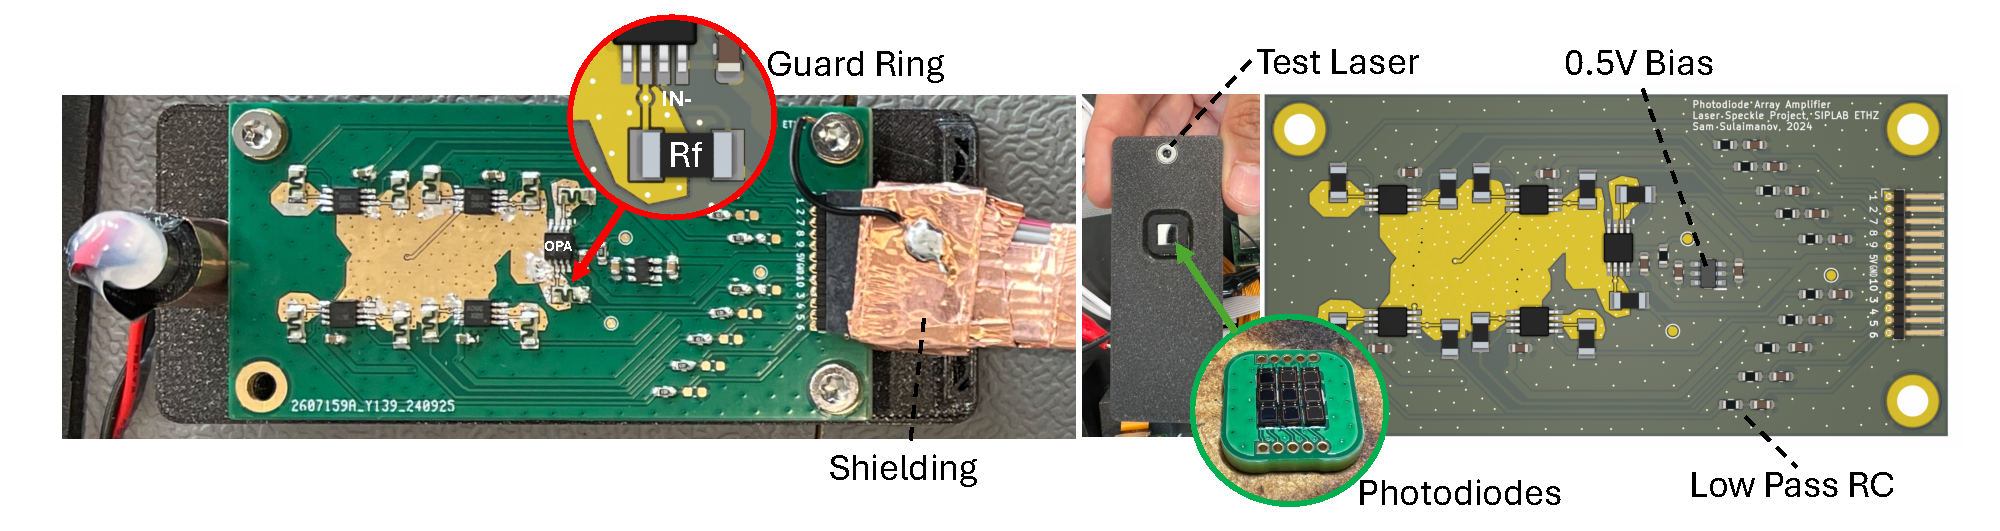
\includegraphics[width=\textwidth]{figures/impl/pcb_design}
    \caption{Left: the final assembled discrete photodetector in a test housing.  Middle: Front view of the detector with IR bandpass filter. Right: Rendered PCB.}
     \label{fig:teaser}
}

\maketitle

% include abstract section
\begin{abstract}
Camera imaging sensors - placed adjacent to a surface diffusing the collimated light of a laser - can be used to sense the resulting surface dependent speckle pattern. The pattern oscillates if the surface oscillates, leading to the possibility of remote vibrometry. While cameras are low cost, easy to use and highly sensitive, they have relatively low frame-rate and thus are thus a poor choice of sensor for high rate oscillations.
The present work explore the creation of a device to increase the measurement bandwidth while maintaining the sensitivity an off the shelf imaging sensor can provide. 
To this end, a high gain low noise amplifier array has been designed with a bandwidth of 1 \si{\kilo\hertz}. The array amplifies the currents of a grid of 3x3 photodiodes which is then low pass filtered and digitized using a high rate ADC.
Tests were conducted to measure the ability of the device to detect laser speckles. Discrete IR lasers, with different beam patterns, and IR dot projectors were evaluated and a detection limit is defined.
\end{abstract}


% Keywords
\keywords{\plainkeywords}

% include all the files into the document
\section{Introduction}
\label{sec:intro}

Vibration sensing enables condition monitoring and predictive maintenance of industrial equipment by detecting mechanical faults before catastrophic failure occurs. 
Critical applications include monitoring of rotating machinery, bearings, and industrial robots, where unexpected downtime can result in significant production losses. 
Higher frequency vibrations are of particular interest \cite{cm-highfreq}.

Typically, a vibration sensor is physically coupled to a designated surface of a machine using adhesive or glue. 
However, this brings the burden of cable management onto the user. Wireless sensors need their batteries replaced once in a while and require a receiving station. 
These limitations motivate the need for a vibration sensor that is easier to install and maintain and capable of monitoring many instances of equipment at once.

Some monitoring approaches use microphones installed centrally in the room, using sound as a proxy for vibration. 
Many microphones are required to distinguish sounds coming from different sources. Remote video cameras can be used to record vibrations \cite{camvibration} when aimed at a fiducial marking. 
Many objects can fit in the field of view of a camera and can thus be monitored. 

While cameras offer a non-contact and simple method for vibration sensing, they're limited to detecting macroscopic (resolution limited) and low-frequency (frame-rate limited) vibrations.
In order to measure microscopic vibrations, we can exploit the speckle patterns that an optically rough surface produces (surface height variations on the order of laser wavelength) 
when laser light (like from a laser pointer) hits it.

When the laser light is reflected and scattered by the optically rough surface, it produces a locally unique and stationary interference pattern. 
This pattern, known as a speckle pattern, results from the superposition of coherent light waves with different path lengths due to the surface's microscopic imperfections. 
The resulting speckle pattern can be observed on any imaging plane at a distance from the surface. To capture this pattern one can expose the bare image sensor (without lens) 
of any camera to the reflected and scattered light.

When the surface is mechanically deformed, the imperfections are altered, causing the pattern to change as well. 
If the surface is translated under the laser light, the pattern appears to shift.

In this work, we exploit this phenomenon for high speed remote vibration sensing. Our approach exceeds the bandwidth limitations of camera-based vibration sensing by capturing 
speckle patterns with an array of discrete high-speed photo-detectors arranged in a 3x3 grid - essentially a discrete image sensor. The novel discrete image sensor combines the advantages of remote, 
non-contact sensing with the ability to capture vibrations at a higher sampling rate than conventional cameras.

To implement this concept, we designed and built the analog photo-detectors on a custom printed circuit board (PCB).

The performance of the hardware was assessed in experiments using laser modules and a laser dot projector at 850 \si{\nano\meter}, 
with surface reflectivity being a critical factor in detection quality. A key finding was that multiple aligned laser sources could be used simultaneously without degrading the signal quality, 
enabling easier aiming from a distance.

Hardware design parameters like pixel size and sensitivity were empirically deduced by using a reference the Raspberry Pi™ HQ camera 12.3 MP (IR filter and objective lens removed) as a reference image sensor.

Detection of genuine speckle patterns was verified through comparative testing against non-coherent LED illumination, which produced no detectable vibration signal.

Our discrete sensor has a bandwidth of 1 \si{\kilo\hertz} exceeding the maximum sampling rate of conventional cameras by an order of magnitude. Our sensor has a comparable sensitivity to the reference sensor. 

\subsection{Contributions}

The work in this semester project makes the following contributions.

\begin{itemize}
    \item High-bandwidth discrete sensor. Developed 1.5 kHz single-supply bandwidth sensor, surpassing conventional cameras by order of magnitude.
    \item Sensitivity optimization. Achieved comparable sensitivity to a reference camera sensor while maintaining high bandwidth.
    \item Laser setups. Produced a variety of low cost laser projector and discrete laser module setups.
    \item SNR improvement. If the sensors sensitivity is high enough for sensing one lasers backscattered light, then increasing the laser beam count improves SNR.
\end{itemize}
\section{Related work}
\label{sec:related_work}

The work in this thesis is related to Laser Speckle Imaging, Laser Doppler Vibrometry and Laser Speckle Vibrometry.

\subsection{Laser Speckle Imaging}
Laser speckle imaging analyses the interference patterns generated when coherent light from a laser, scatters off an optically rough surface. 
These "speckles" can be captured by any photosensitive surface - and most commonly - a camera image sensor. 
The mean speckle size is an important parameter, as the pixels of the image sensor must be smaller in order to resolve a pattern. 
The speckle size is a statistical property of the interference pattern and depends on the laser wavelength, sensor-to-surface distance and illuminated area. 
Cloud \cite{specklesize} defines the speckle size as "the center-to-center spacing of adjacent dark or adjacent light spots in the speckle pattern". 

It can be expressed approximately:
\[
\text{Mean speckle size} \approx \lambda \cdot \frac{d}{\sqrt{a}}
\]
where:
\begin{itemize}
    \item \(\lambda\) is the wavelength of the laser light,
    \item \(d\) is the distance from the scattering surface to the observation plane,
    \item \(a\) is the diameter or size of the illuminated area (e.g. laser spot area).
\end{itemize}

Hu et al. \cite{specklesizeANDstructure} show that the size of the speckle is not impacted by the structure of the laser beam.
Using multiple lasers increases the illuminated area and reduces the speckle size. \ref{fig:speckles}

Speckle size can be tuned without changing $d$ or $a$ by de-focused imaging, proposed by Heikkinen and Schajer \cite{defocusedVSobjective}.
They use a de-focused telephoto lens to optically change $d$ and show that the resulting speckle pattern is comparable if $d$ was changed physically.
The method has an additional advantage of sampling a larger speckle field and capturing more light, important for weaker signals.

Laser speckle imaging is simple to implement and does not require significant hardware, which motivates this semester project.
Yan et al. \cite{lasershoes} developed "LaserShoes," a system using a USB webcam and Raspberry Pi mounted on shoes to classify ground textures based on speckle patterns.
They evaluated different laser wavelengths and achieved accurate surface recognition with a compact, low-cost system. 
Chan et al. \cite{milkdrop} measured liquid characteristics (e.g., milk fat content) using smartphone LIDAR to image speckles, 
though many frames were needed due to the low power of the LIDAR laser.


\subsection{Laser Doppler Vibrometry}

Laser Doppler Vibrometry (LDV) measures an objects velocity by detecting the Doppler shift in the frequency of reflected coherent light. 
The measurement setup required is more complex as it involves mixing the emitted and back scattered laser light to detect a beat frequency, 
which if proportional to the velocity \cite{LDVreview}. LDV offers high precision and can measure large vibrations, but the complex setup makes it costly and challenging to scale. 
Speckle noise is a known limitation in LDV, caused by random phase shifts in scattered light due to surface roughness. 
Addressing this noise often requires advanced signal processing \cite{LDVreview}.

\subsection{Laser Speckle Vibrometry}

Laser Speckle Vibrometry detects vibrations from changes in the speckle pattern over time. 
Unlike LDV, it is much simpler, requiring only at least 1 photodiode or camera to capture intensity changes.

Veber et al. \cite{veber2011laserMASK} used a single photodiode with a spatial mask and telephoto lens. 
Their system was able to measure vibrations at distances up to 50 m using a high power (1.5 W) laser. 
It detected oscillations of a sheet of paper exposed to sound pressure at 50 dB up to 5 kHz. On the other hand, 
Streli et al. \cite{structured-light-speckle} demonstrated a camera-based method using a 200 FPS camera with laser 
pointer modules to detect finger taps on a surface. However, the limitations of camera frame rates restrict detection to lower frequencies.

Speckle vibrometry is effective for small-amplitude vibrations (including translation and pitch) but struggles with vibrations parallel 
to the laser beam (where LDV excels). Its simplicity and cost-effectiveness make it an attractive alternative to LDV for lower-cost applications.
\section{Implementation}
\label{sec:implementation}

\subsection{System Design}

Backscattered light from an object hit by a laser, like a speckle pattern, is typically very low in intensity. How low depends on the situation.

The light intensity $I_b$ at a distance $d$ is proportional to the laser power and decays quadratically with distance and can be calculated using a simplified model:

\begin{equation}
I_b = \frac{P \cdot \rho}{2\pi d^2},
\end{equation}
where:
\begin{itemize}
\item $P$ is the power of the incident laser beam, measured in watts (W),
\item $\rho$ is the reflectivity of the surface (unitless),
\item $d$ is the distance from the scattering surface to the photodiode, measured in meters (m).
\end{itemize}


\subsection{How much current?}
A photodiode converts the backscattered light intensity into current:
\begin{equation}
I_{\text{photo}} = I_b \cdot A_{\text{PD}} \cdot R,
\end{equation}
where:
\begin{itemize}
\item $I_b$ is the incident intensity at distance $d$ \text{(W/mm\textsuperscript{2})},
\item $A_{\text{PD}}$ is the area of the photodiode \text{(mm\textsuperscript{2})},
\item $R$ is the photodiode responsivity \text{(A/W)}.
\end{itemize}
Using typical values like $R = 0.5\text{A/W}$, $A_{\text{PD}} = 2\text{ mm}^2$, $P = 1\text{ mW}$ and $d = 0.3\text{ m}$ we are left with tiny photocurrents in the $500\text{ pA}$ range!

To be certain, we conduct a small set of experiments (setup is shown in Figure \ref{fig:cam1}) to measure the current produced by a photodiode exposed to incident laser speckle pattern.

A typical store-bought class 1 red laser pointer has an output power under 0.5mW. 
Using this laser pointer and the Thorlabs PDA36A2 photodetector (with a photodiode area: $A_{\text{PD}} = 13\text{ mm}^2$ and same $d$ as above), we observe ~13 ~nA of current.
This means that we need to at least be able to measure currents on this order of magnitude for class 1 lasers at ~30 ~cm distance.


\subsection{How big a photodiode?}
Can we test if a photodiode of a given size can be sensitive to a speckle pattern in motion? Recall that the sensor must be smaller than the speckle size in order to resolve speckle motion. Using the formula for mean speckle size, assuming a red laser at 650 ~nm and 30 ~cm distance, we find the resulting mean size to be around 100 ~um. This is smaller than common photodiodes. We make the assumption - based on observations of real speckle patterns - that the variance in size is large. That means that some speckles will be on the order of a common small photodiode ($1\text{ mm}^2$), meaning that we will be able to sense a variance in intensity when speckles pass over the photodiode.

To validate this assumption, we masked the detector with a 0.9mm x 0.9mm pinhole (poked a hole, then measured it) on copper tape to cover the aperture of the detector (inspired by \cite{veber2011laserMASK}). 
We set the surface in motion and observed the output on a multimeter as well as on camera. As the speckle oscillated on camera, so did the multimeter output.

With this, we find the most sensitive, small, low cost photodiode on Digikey: the VEMD2704 by Vishay with an area of $1.5\text{ mm}^2$.

\subsection{How many photodiodes?}
We know we can detect the speckle pattern translation with 1 photodiode. And while we can calculate the mean speckle size, we have no grasp of its variance with just one photodiode. If we arrange multiple photodiodes in a grid, some of them will see darker spots and some will see lighter spots. This means that given a grid of photodiodes, we can detect the global change in speckle pattern variance. 

We use the Raspberry Pi HQ camera sensor to determine the spacing and size of the grid experimentally.

We make the following observations:
\begin{itemize}
  
  \item A CMOS sensor pixel is a photodiode and has as determined size.
  \item We can emulate the output of a larger photodiode by integrating over all pixels over the same area as the larger photodiode.
  \item The sensor area of the RPI camera is large enough to accommodate 9 VEMD2704 photodiodes (see Figure \ref{fig:emulated2}).
\end{itemize}

Using this knowledge, we record a video of a speckle pattern in motion and cut out the pixels corresponding to a grid of areas the same sizes as the VEMD2704.
We establish that an algorithm similar to the one used by Streli et al \cite{structured-light-speckle} can be used to combine the outputs of the photodiodes in order to create a 1d motion signal.
Figure \ref{fig:emulated2} shows the resulting 1d signal of motion (essentially speckle pattern variance). The section on Signal Processing discusses this in detail.

In fact, in the camera experiments we only simulated a horizontal grid of 3 VEMD2704 photodiodes. Using a 3x3 grid would theoretically allow direction sensing, but this was not tested. A 3x3 grid also increases SNR as we have more samples to compute the speckle variance.

\subsection{Hardware Implementation}
We want a simple and cost effective solution, to amplify and digitize the photodiode signals, that is flexible enough for experimentation.
A single amplifier stage is chosen that is directly coupled, through an antialiasing filter, to an analog to digital converter (ADC). 

Photodiodes are commonly amplified using a transimpedance amplifier (TIA), or a current to voltage amplifier. Although alternative options exist, such as current integrators like the DDC118, they require more complex setups and control.

The TIA current to voltage gain and bandwidth is defined by the the feedback path.

\begin{equation}
V_{\text{out}} = R_f \cdot I_{\text{in}},
\end{equation}
where:
\begin{itemize}
\item $V_{\text{out}}$ is the output voltage (V)
\item $R_f$ is the feedback resistance ($\Omega$)
\item $I_{\text{in}}$ is the input current (A)
\end{itemize}

\begin{equation}
f_{-3\text{dB}} = \frac{1}{2\pi R_f C_f},
\end{equation}
where:
\begin{itemize}
\item $f_{-3\text{dB}}$ is the -3dB bandwidth (Hz)
\item $R_f$ is the feedback resistance ($\Omega$)
\item $C_f$ is the feedback capacitance (F)
\end{itemize}

We want a gain that supports a good range of AC and DC photocurrent. We assume that we will have 1nA peak-to-peak AC induced by a IR speckle pattern in motion. No analog DC rejection is performed, to keep things simple, so we must account for microamps of potential DC photocurrent. If we use a 100 MOhm feedback resistor, we can achieve 100 mV AC output. In order to not saturate the opamp with DC current, filtering the input light with an IR bandpass filter is a must. For indoor purposes, there is practically no IR content in typical LED office lighting, though rooms with lots of natural light would still pose problems. From the power vs spectrum graphs of white LEDs, we deduce that at 850nm the VEMD2704 would output around 10nA of current - not saturating our opamp.

The bandpass filter is chosen to be IR at 850nm as that is conveniently where silicon photodiodes are most efficient. Lasers at 850nm are also very common.
 
To maximise possible bandwidth, we choose a minimal amount of feedback capacitance, which is just the stray capacitance coming from the feedback resistor (0.2 pF). Using the above formula, the amplifier bandwidth is 7.9 kHz. 

We now use the feedback path and photodiode parameters in Formula 10 of \cite{TIABW}, to calculate a required GBW (gain bandwidth product) for guaranteed amplifier stability. We find that we must choose an operational amplifier with more than 1110 kHz of GBW.

For a simple experimental setup, we want to use a Raspberry Pi for data processing, recording and visualisation. Many relatively high speed and low cost ADCs exist for the Raspberry Pi, that are easily read out via Python. The data rates are on the order of 1-10kSPS per channel.

We test two ADCs in this project:
\begin{itemize}
  \item Waveshare High-Precision AD HAT (ADS1263): 10 channel mux, 1 ADC with 32-Bit resolution, 38400 SPS (total).
  \item Digilent MCC128: 8 channel mux, 1 ADC with 16-bit resolution, 100 kSPS (total).
\end{itemize}
Both are multichannel ADCs that use a multiplexer to switch between all channels. 

The first ADC was unable to sample at high enough frequencies. The channel switching is controlled via SPI, making it challenging to manage the switching delay and the effective sample rate. This mux also produced a significant amount of noise, even with filtering, which was noted in several GitHub issues reported by users. Only a low sample rate of around 200 Hz was achieved.

The second ADC was then tested, featuring a higher sample rate and advertised synchronous sample readout capability. Unfortunately this ADC inexplicably uses the Pi's 5V supply as its analog reference. However, this is very noisy, with peak-to-peak noise in the millivolt range. To mitigate this issue, a bench power supply was used to power the ADC externally. Stable sampling frequency of 4kHz per channel could be achieved.

We limit the bandwidth of the amplifier stage to 1.5~kHz (half the sample rate of the first ADC) with an RC low pass filter. This is done to prevent aliasing noise in the ADC.

We devise a system block diagram in Figure \ref{fig:block}.

\begin{figure}[t]
  \centering
  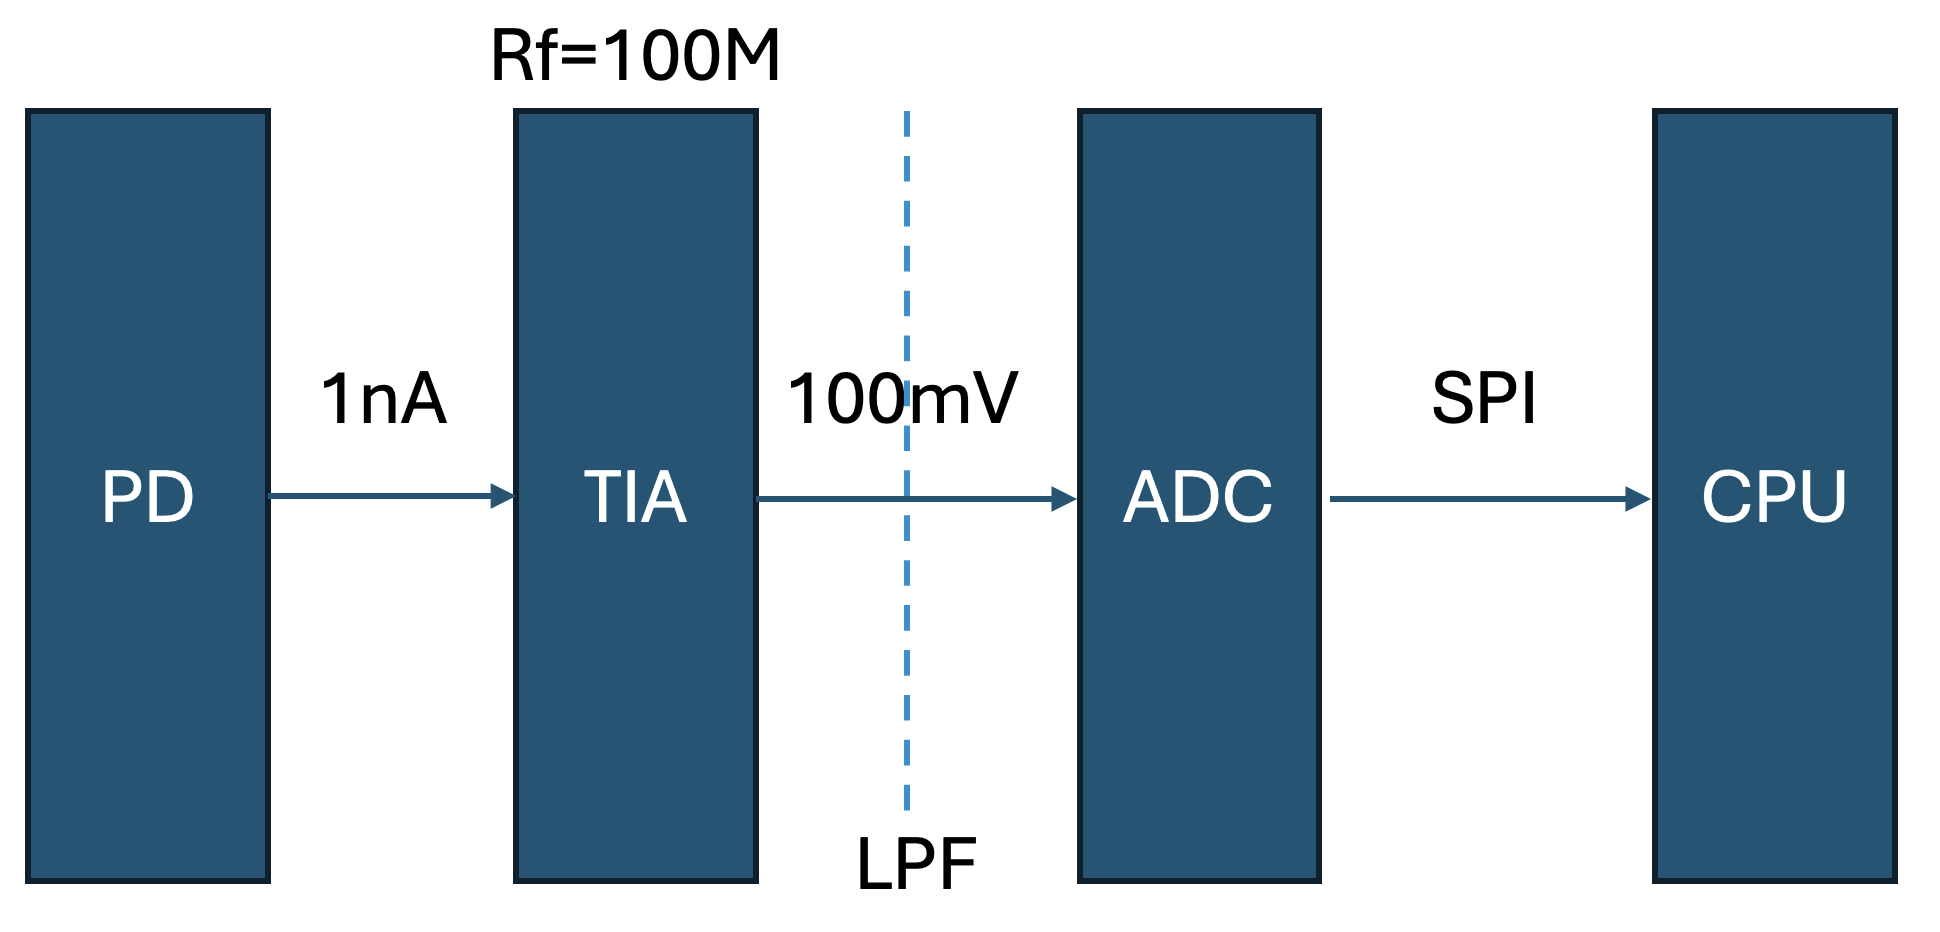
\includegraphics[width=\widthnarrow]{figures/impl/block_diagram.png}
  \caption{Block diagram}
  \label{fig:block}
\end{figure}

The essential requirements for the op-amps include:
\begin{itemize}
  \item A minimum of two op-amps in a single package.
  \item A target price of approximately \$5 per chip.
  \item JFET input with low input bias current.
  \item Low noise, low voltage offset and low voltage offset drift.
  \item Capability to operate on a single power supply.
  \item To guarantee stability, it must have a GBW of at least 1100 kHz.
\end{itemize}

The OPA2380 fulfills these requirements and a PCB was designed and built according to the datasheet recommendations. The simplified schematic is given in Figure \ref{fig:spice}.

\begin{figure}[t]
\centering
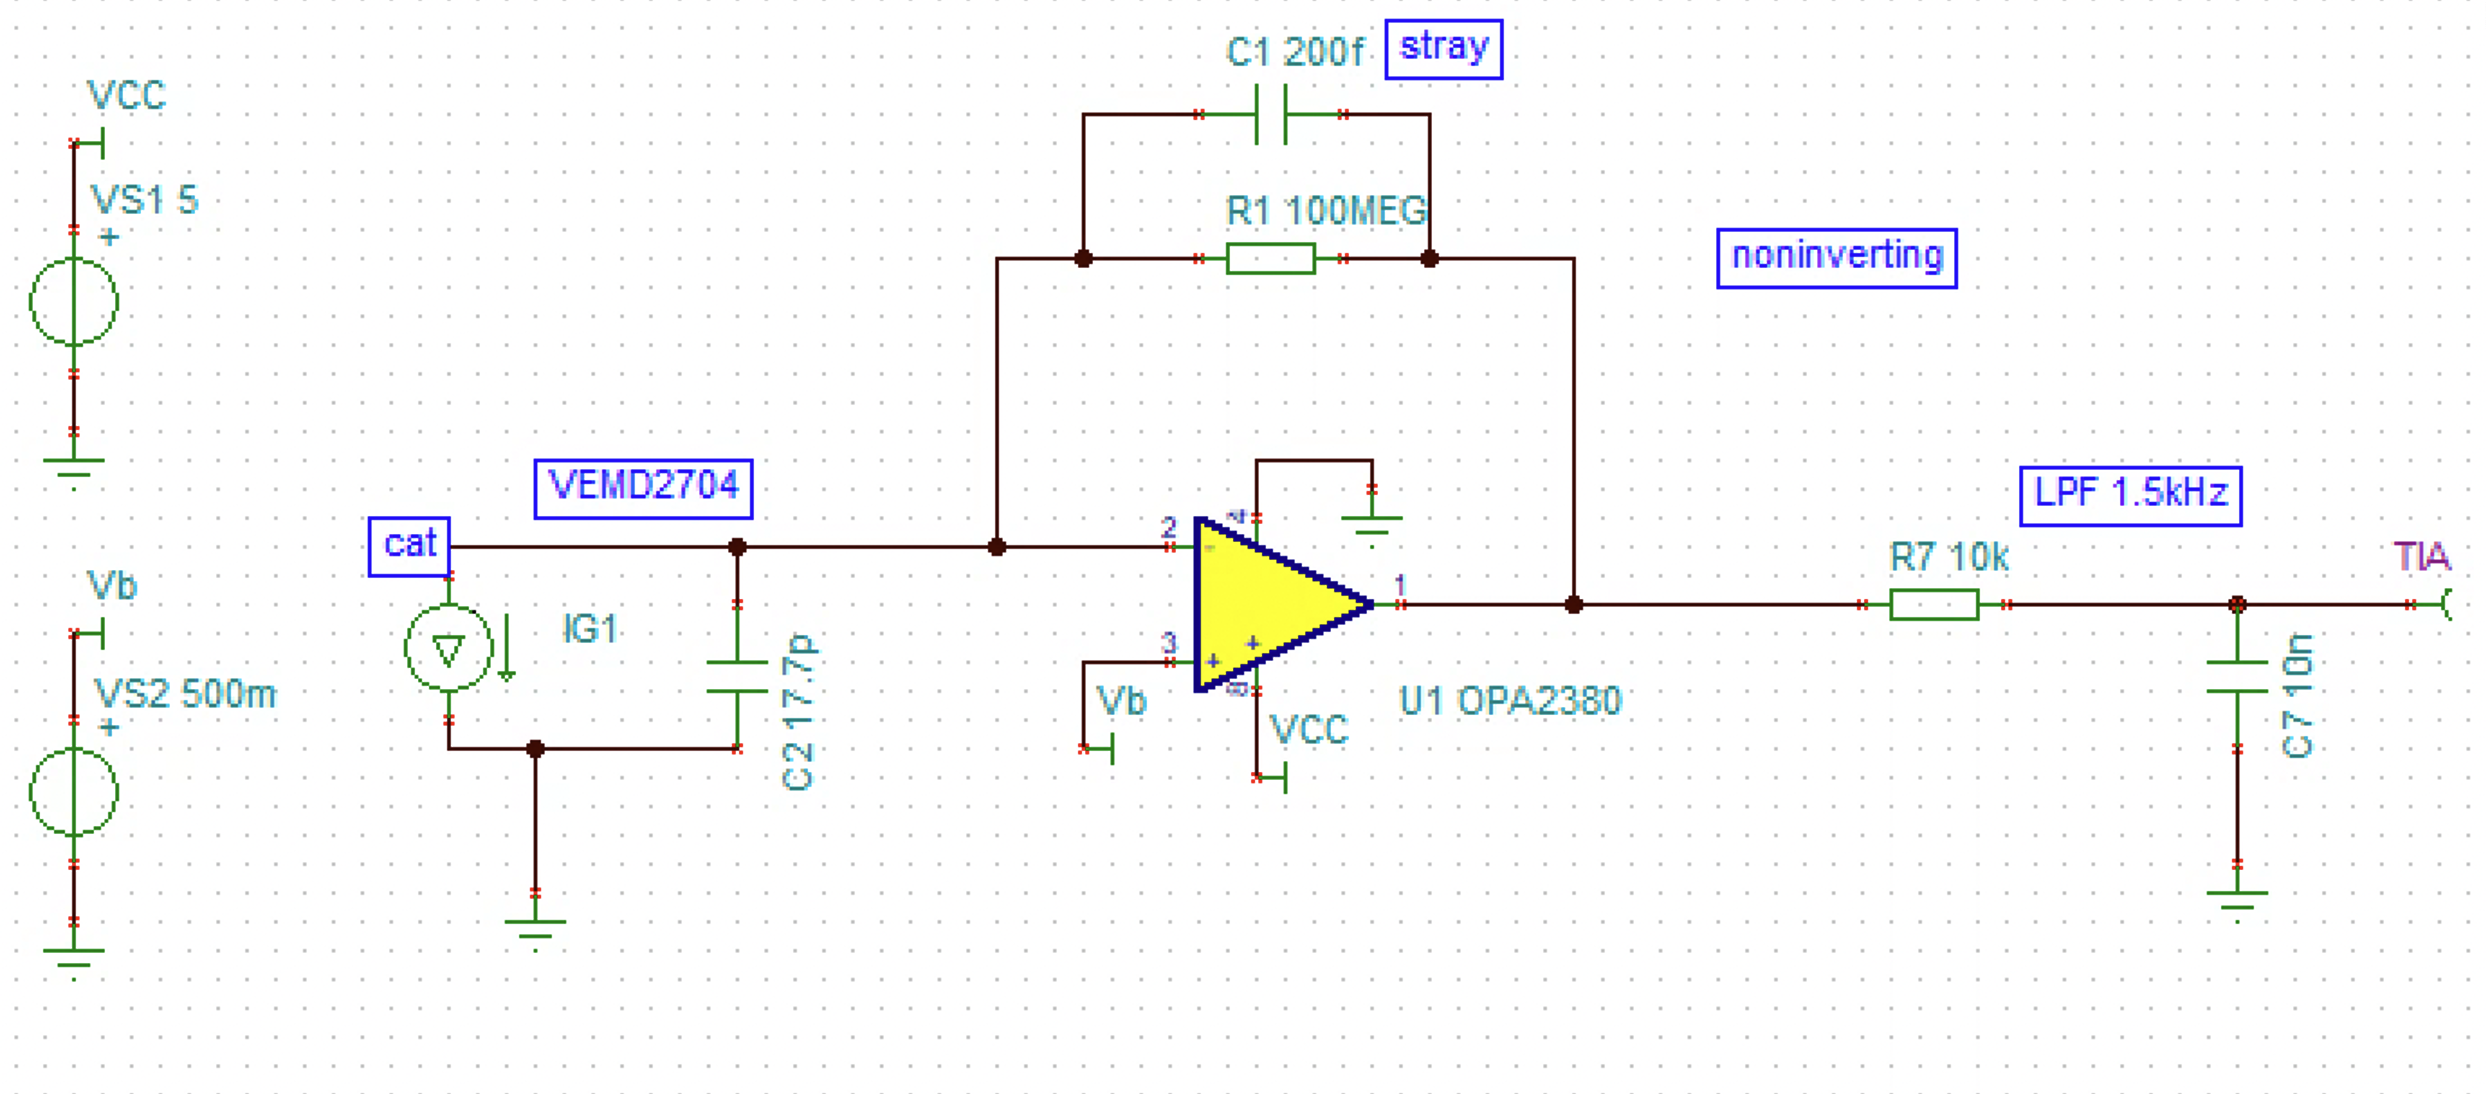
\includegraphics[width=\widthnarrow]{figures/eval/spice.png}
\caption{Amplifier schematic with equivalent photodiode (VEMD2704) and output filter.}
\label{fig:spice}
\end{figure}
      
Particular attention to leakage currents in the feedback path was taken, like the implementation of a guard ring. The guard ring is a low impedance path for any stray AC that might want to make its way into the feedback path of the amp. The PCB is shown in Figure \ref{fig:teaser} and contains a modular photodiode array with bandpass filter.


\subsection{Signal Processing}
To convert the 9-channel photodiode array readings into a single vibrometry signal, we compute the inter-channel variance, explained later on. 
First, we remove common-mode fluctuations by subtracting the instantaneous mean across all channels:

\begin{equation}
s_i(t) = r_i(t) - \frac{1}{n}\sum_{k=1}^{n} r_k(t)
\end{equation}

where $r_i(t)$ is the raw intensity reading from channel $i$ and $n=9$ is the number of channels. We then compute the inter-channel variance:

\begin{equation}
V(t) = \frac{2}{n(n-1)} \sum_{i=1}^{n-1} \sum_{j=i+1}^{n} |s_i(t) - s_j(t)|
\end{equation}

This metric quantifies the average magnitude of pairwise intensity differences between spatial channels in the instantaneous speckle pattern. 
Changes in $V(t)$ over time indicate surface motion and vibration while being robust to common-mode noise.

Raw data from the ADC was recorded and observed in real-time or processed post-capture. 
Real-time observations were conducted while simultaneously monitoring the speckle camera and the infrared (IR) camera.

\begin{figure*}[t]
  \centering
  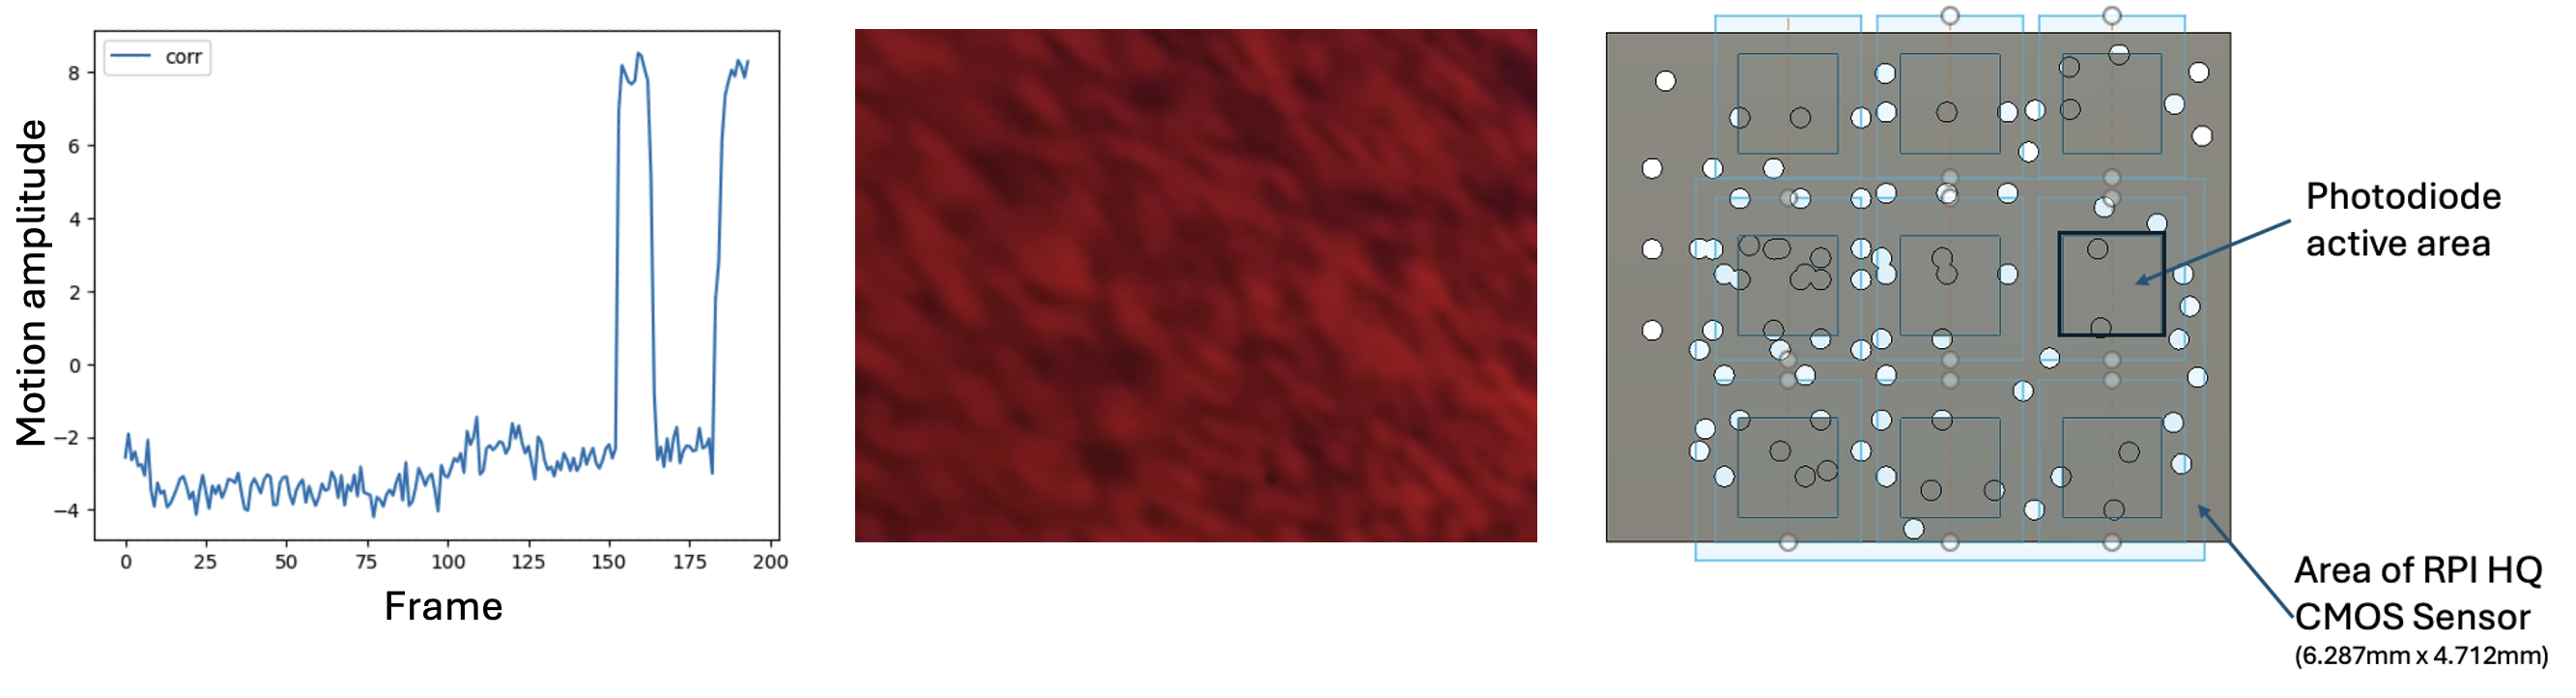
\includegraphics[width=\textwidth]{figures/impl/emulated2.png}
  \caption{Left to right: Peaks show translation of speckle pattern, signifying a change of the inter-channel variance. The speckle pattern on the camera sensor. The camera sensor with an overlayed photodiode grid.}
  \label{fig:emulated2}
\end{figure*}

\subsection{Lasers}

Several laser sources were built in different configurations as seen in Figure~\ref{fig:lasers}. 
The laser module used for the square array, circular array and single laser measurements is an 850~nm laser (VLM-850-03 by Quarton Inc.).
The Realsense D415 Depth Camera (by Intel) has a laser dot projector that can be turned on using the Realsense Viewer Software. 
To control the amount of laser dots that are output by the Realsense dot projector, an iris diaphragm (Edmund Optics 53906) is used.

Additionally, we reverse engineered the Realsense through visual inspection and found it to look very similar, if not identical, to the BELICE projector module by ams. 
To confirm this theory, we measured the laser output power with an integrating sphere on optical power meter (the Artifex OPM150) and found a similar nominal output power of 250 ~mW per module.
As a proof of concept for potential future experiments, a small driver circuit was built based on the example in the LT1800 opamp datasheet \cite{lt1800}. 
\section{Evaluation}
\label{sec:evaluation}

\subsection{Hypotheses}
The primary hypothesis is that the motion of speckle patterns can be effectively visualized using a photodiode array. 
Additionally, it is hypothesized that the use of multiple lasers will influence the signal-to-noise ratio (SNR) of the measurements.

\subsection{Apparatus}

The custom-designed PCB transmitted its analog signals to an 8-channel Digilent ADC MCC 128 DAQ Hat, which was powered by a 5V low-noise bench power supply. 
A piezo disc, positioned at a distance of approximately 30~cm, was excited using a signal generator set to produce a sine wave at 133~Hz with a peak-to-peak amplitude of 3~V. 
All lasers utilized in the setup operated at a wavelength of 850~nm.

For visual alignment of the lasers, one camera was employed, while another camera was used to monitor the presence of speckles. 
Both the cameras and the photodiode array were equipped with 8~$\times$~8~$\times$~1~mm bandpass filters at 850~nm with a 40~nm FWHM and a 90\% transmission rate (manufacturer: Haian Subei Optical Glass Factory).
Data acquisition was handled by a Raspberry Pi, which recorded the ADC data. 
Data processing was performed in real time during qualitative experiments or recorded for later post-processing.

\begin{figure}[t]
\centering
\includegraphics[width=\widthnarrow]{figures/eval/typical_setup.png}
\caption{Photo of the experimental configuration with the piezo disc.}
\label{fig:setup}
\end{figure}

\subsection{Procedure}

The initial steps of the evaluation involved SPICE simulations to analyze the Bode plot and transient response of the amplifier, as illustrated in Figures~\ref{fig:bodeplot} and \ref{fig:transient}. 
These simulations provided the theoretical SNR and total noise values (Figures~\ref{fig:totalnoise} and \ref{fig:snr}), demonstrating that the amplifier displayed stable behavior with high gain. 
Based on these results, the PCB was constructed.

Following the PCB assembly, it was meticulously cleaned using isopropyl alcohol (IPA) and compressed air, particularly under the pads of the amplifier section. 
Removing all flux residue from the PCB was deemed critical to ensure accurate operation. All measurements were conducted in a light-controlled environment to minimize interference from external light sources.

To assess the influence of multiple laser sources, a controlled surface vibration of the piezo disc at 133~Hz was measured while lasers in the square array were activated incrementally (Figure~\ref{fig:lasers}). 
For each configuration, the power spectral density of the inter-channel variance signal was calculated, and the SNR was analyzed. The spectral analysis, shown in Figure~\ref{fig:laser_snr}, 
established a positive correlation ($R^2 = 0.60$) between the number of active lasers and the detection SNR. 
A control measurement with all lasers switched off confirmed that the recorded signals originated from laser speckle patterns.

Additionally, time-domain signals captured by multiple photodiodes were compared to verify that each photodiode detected phase-shifted signals, which indicated the presence of a moving speckle pattern. 
An infrared (IR) LED was integrated into the setup to validate that the observed vibrations were dependent on coherent light.

\begin{figure}[t]
\centering
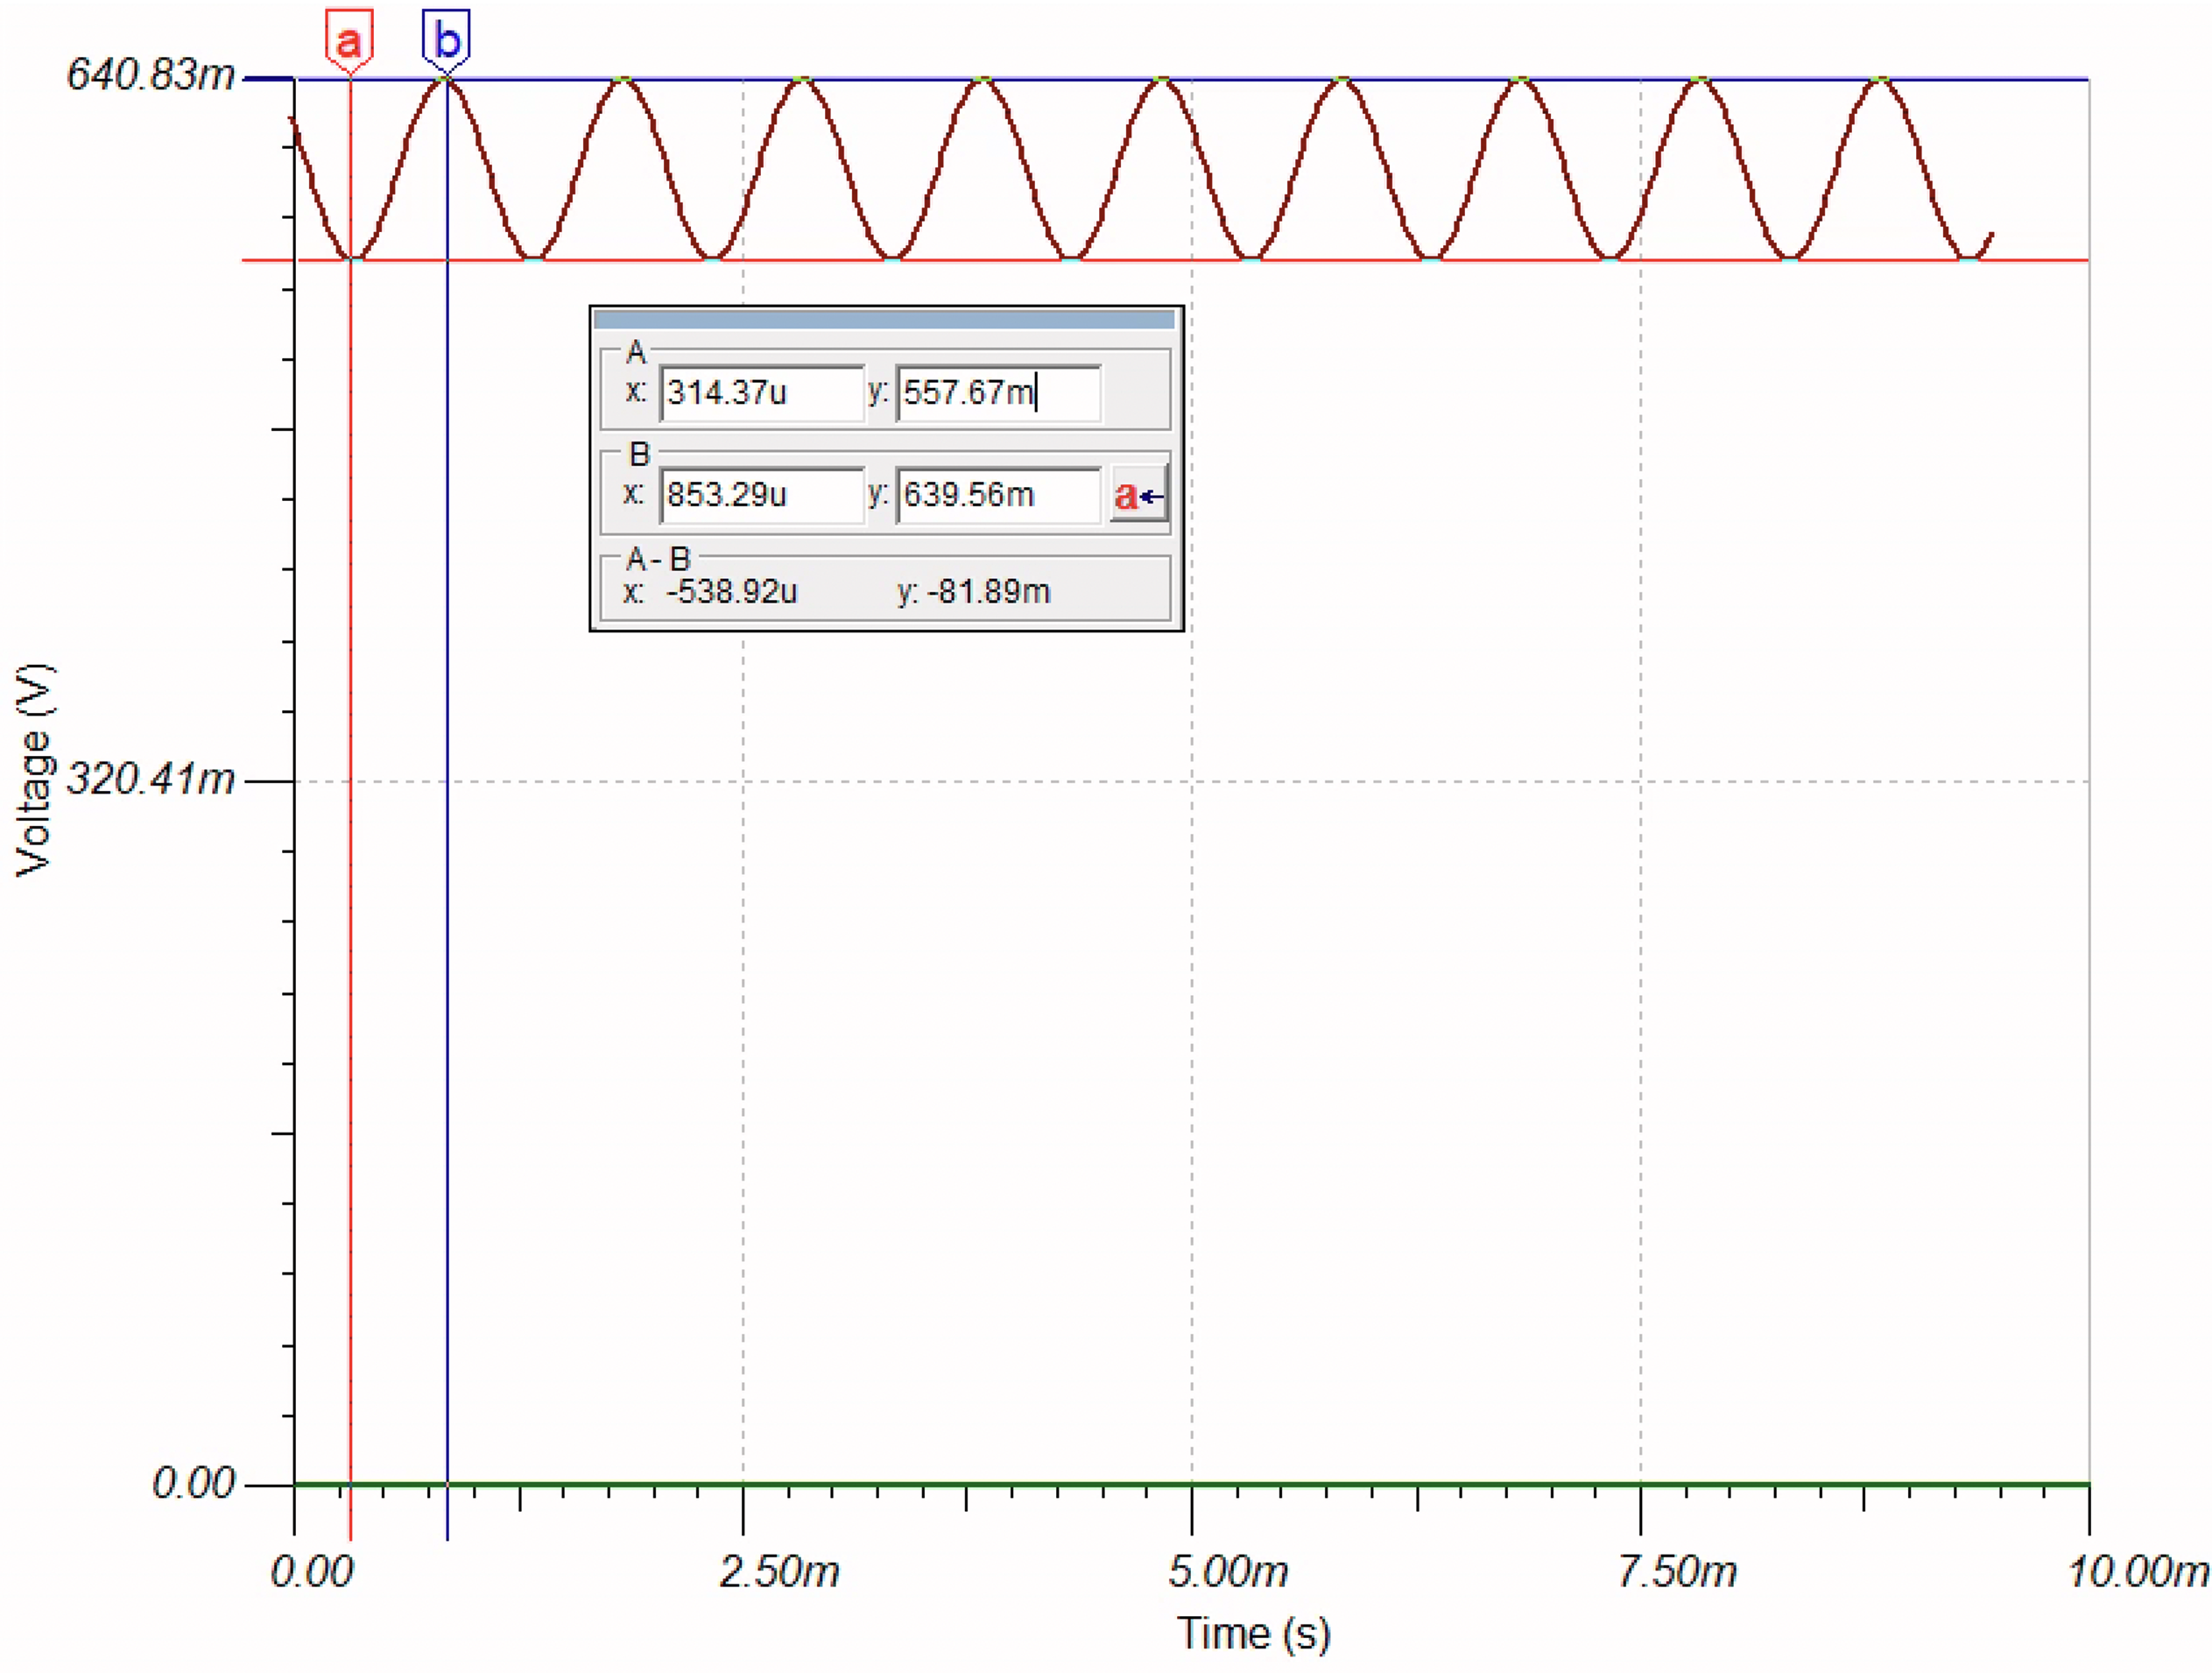
\includegraphics[width=\widthnarrow]{figures/eval/transient}
\caption{Transient response captured during SPICE simulation, highlighting amplifier dynamics and stability.}
\label{fig:transient}
\end{figure}

\begin{figure}[t]
\centering
\includegraphics[width=\widthnarrow]{figures/eval/bode.png}
\caption{Amplifier frequency and phase response.}
\label{fig:bodeplot}
\end{figure}

\begin{figure}[t]
\centering
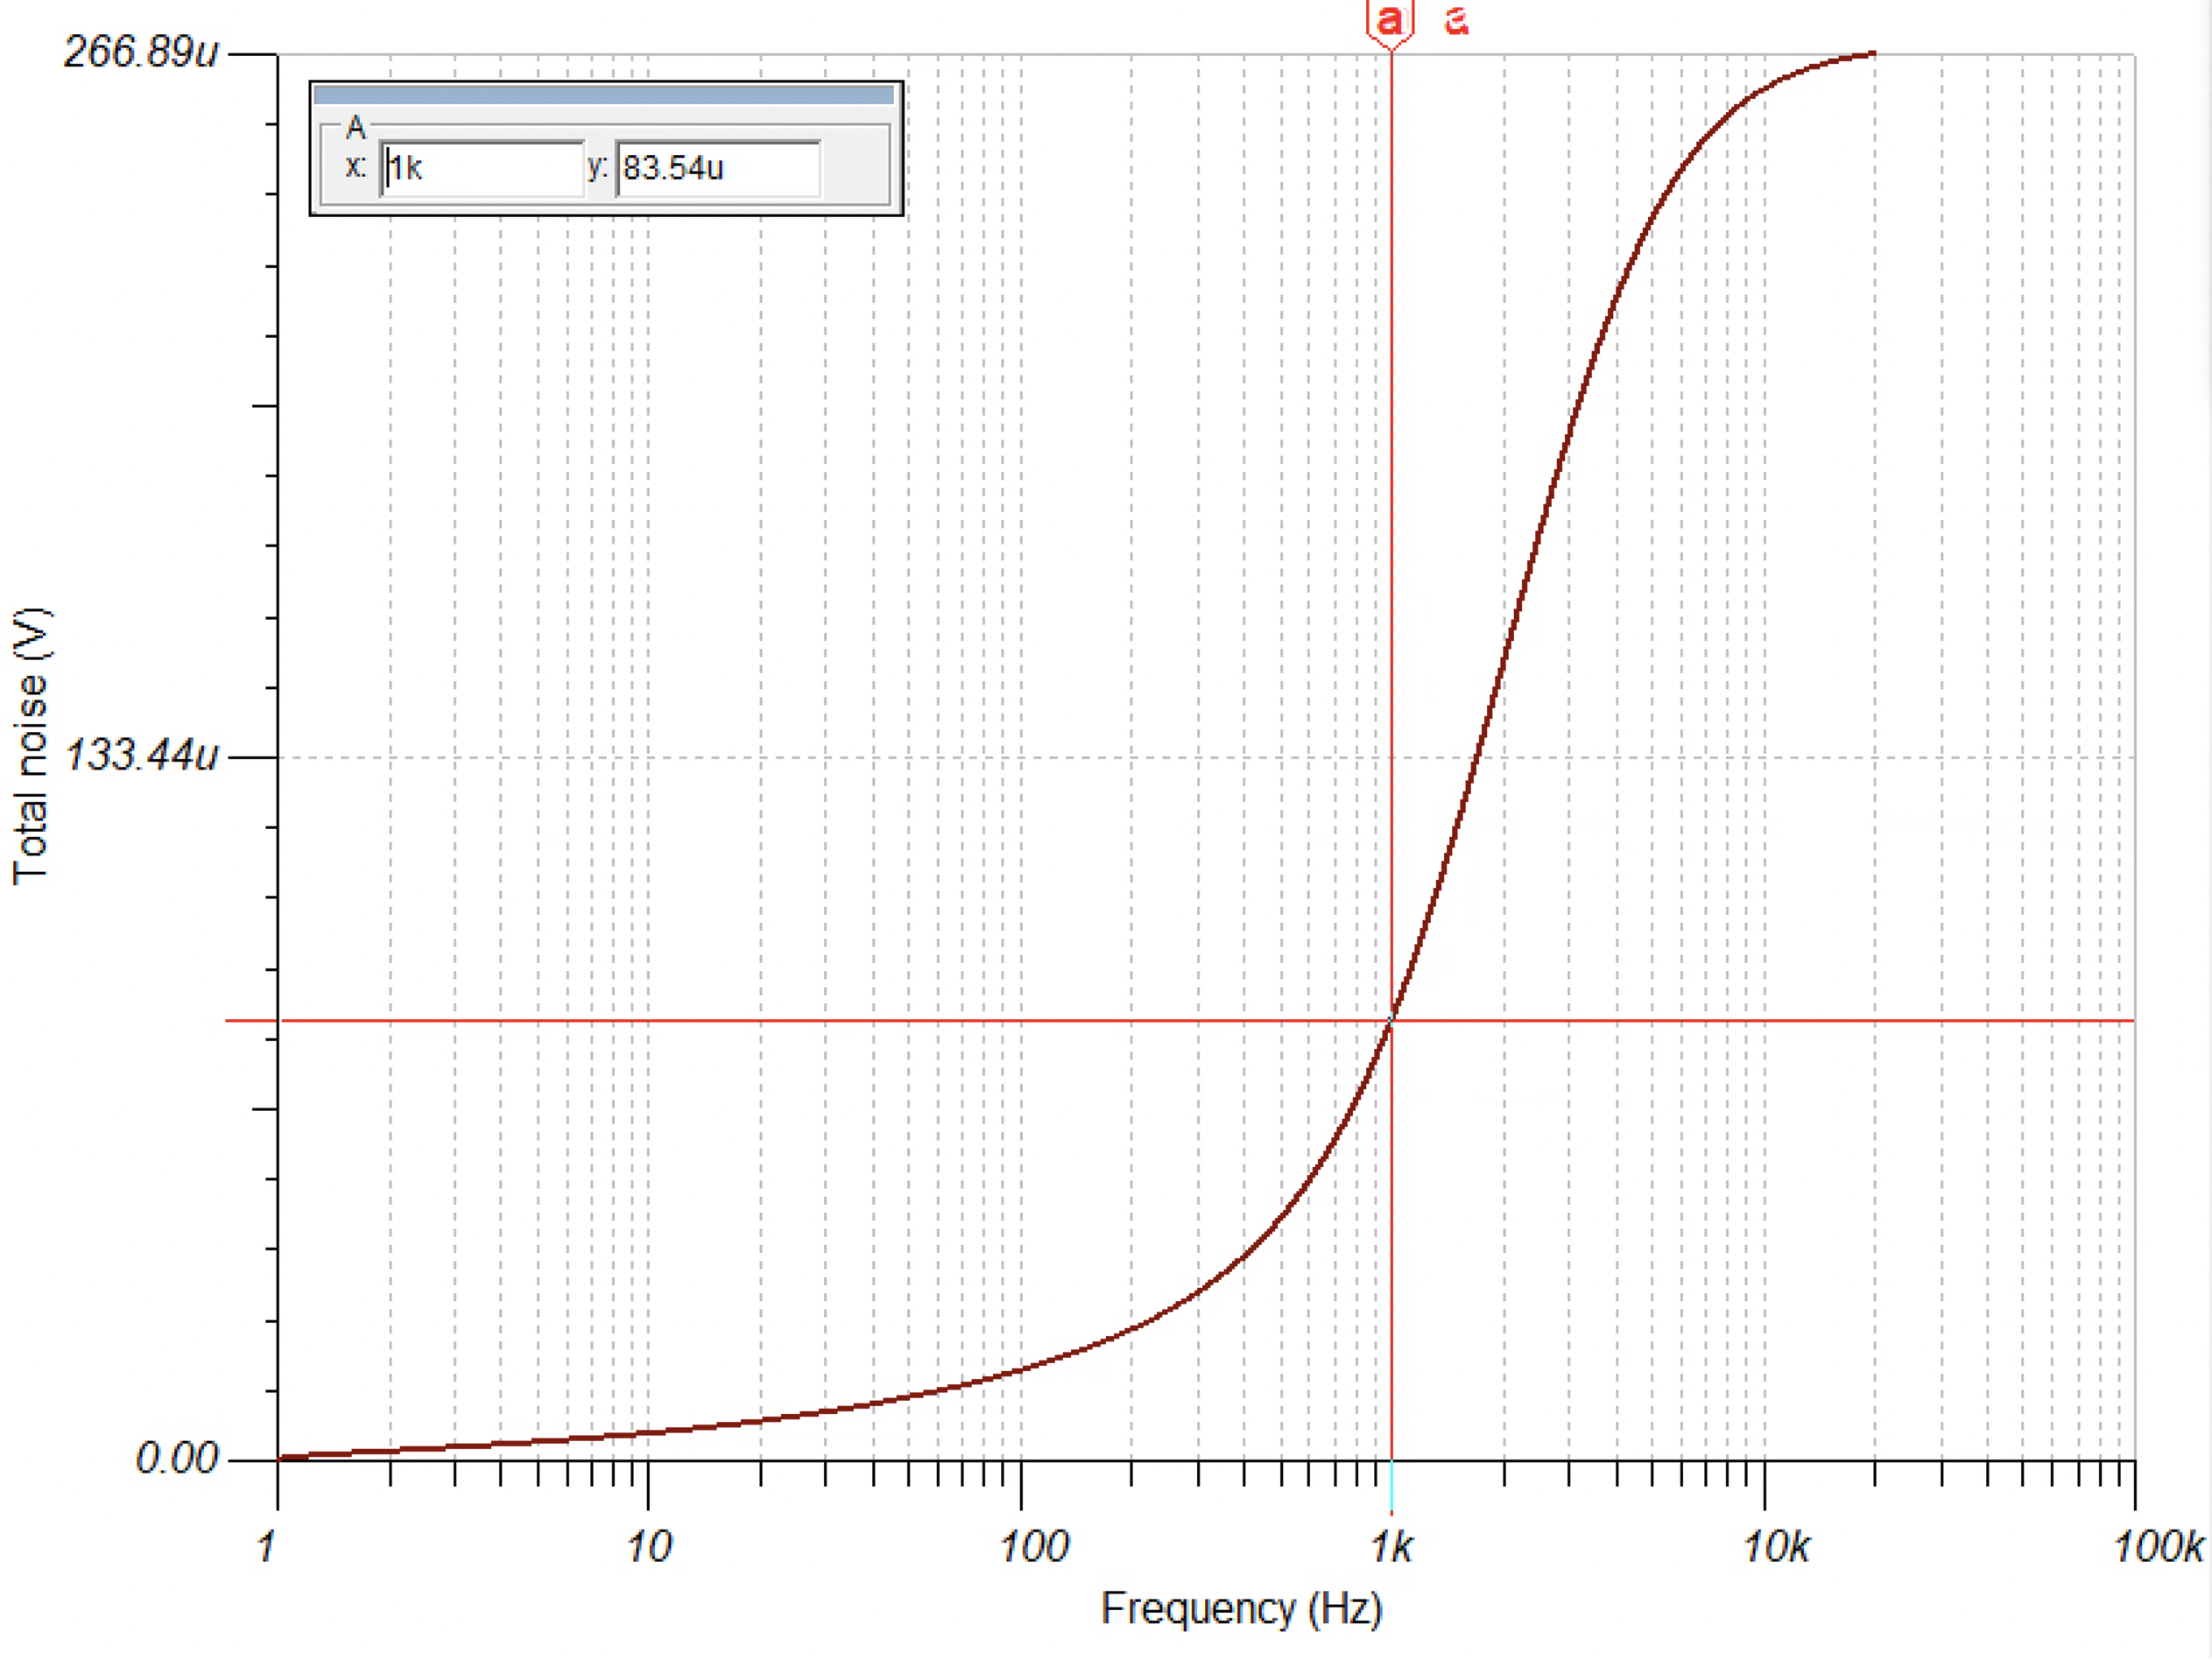
\includegraphics[width=\widthnarrow]{figures/eval/totalnoise.png}
\caption{Total noise of the amplifier vs frequency.}
\label{fig:totalnoise}
\end{figure}

\begin{figure}[t]
\centering
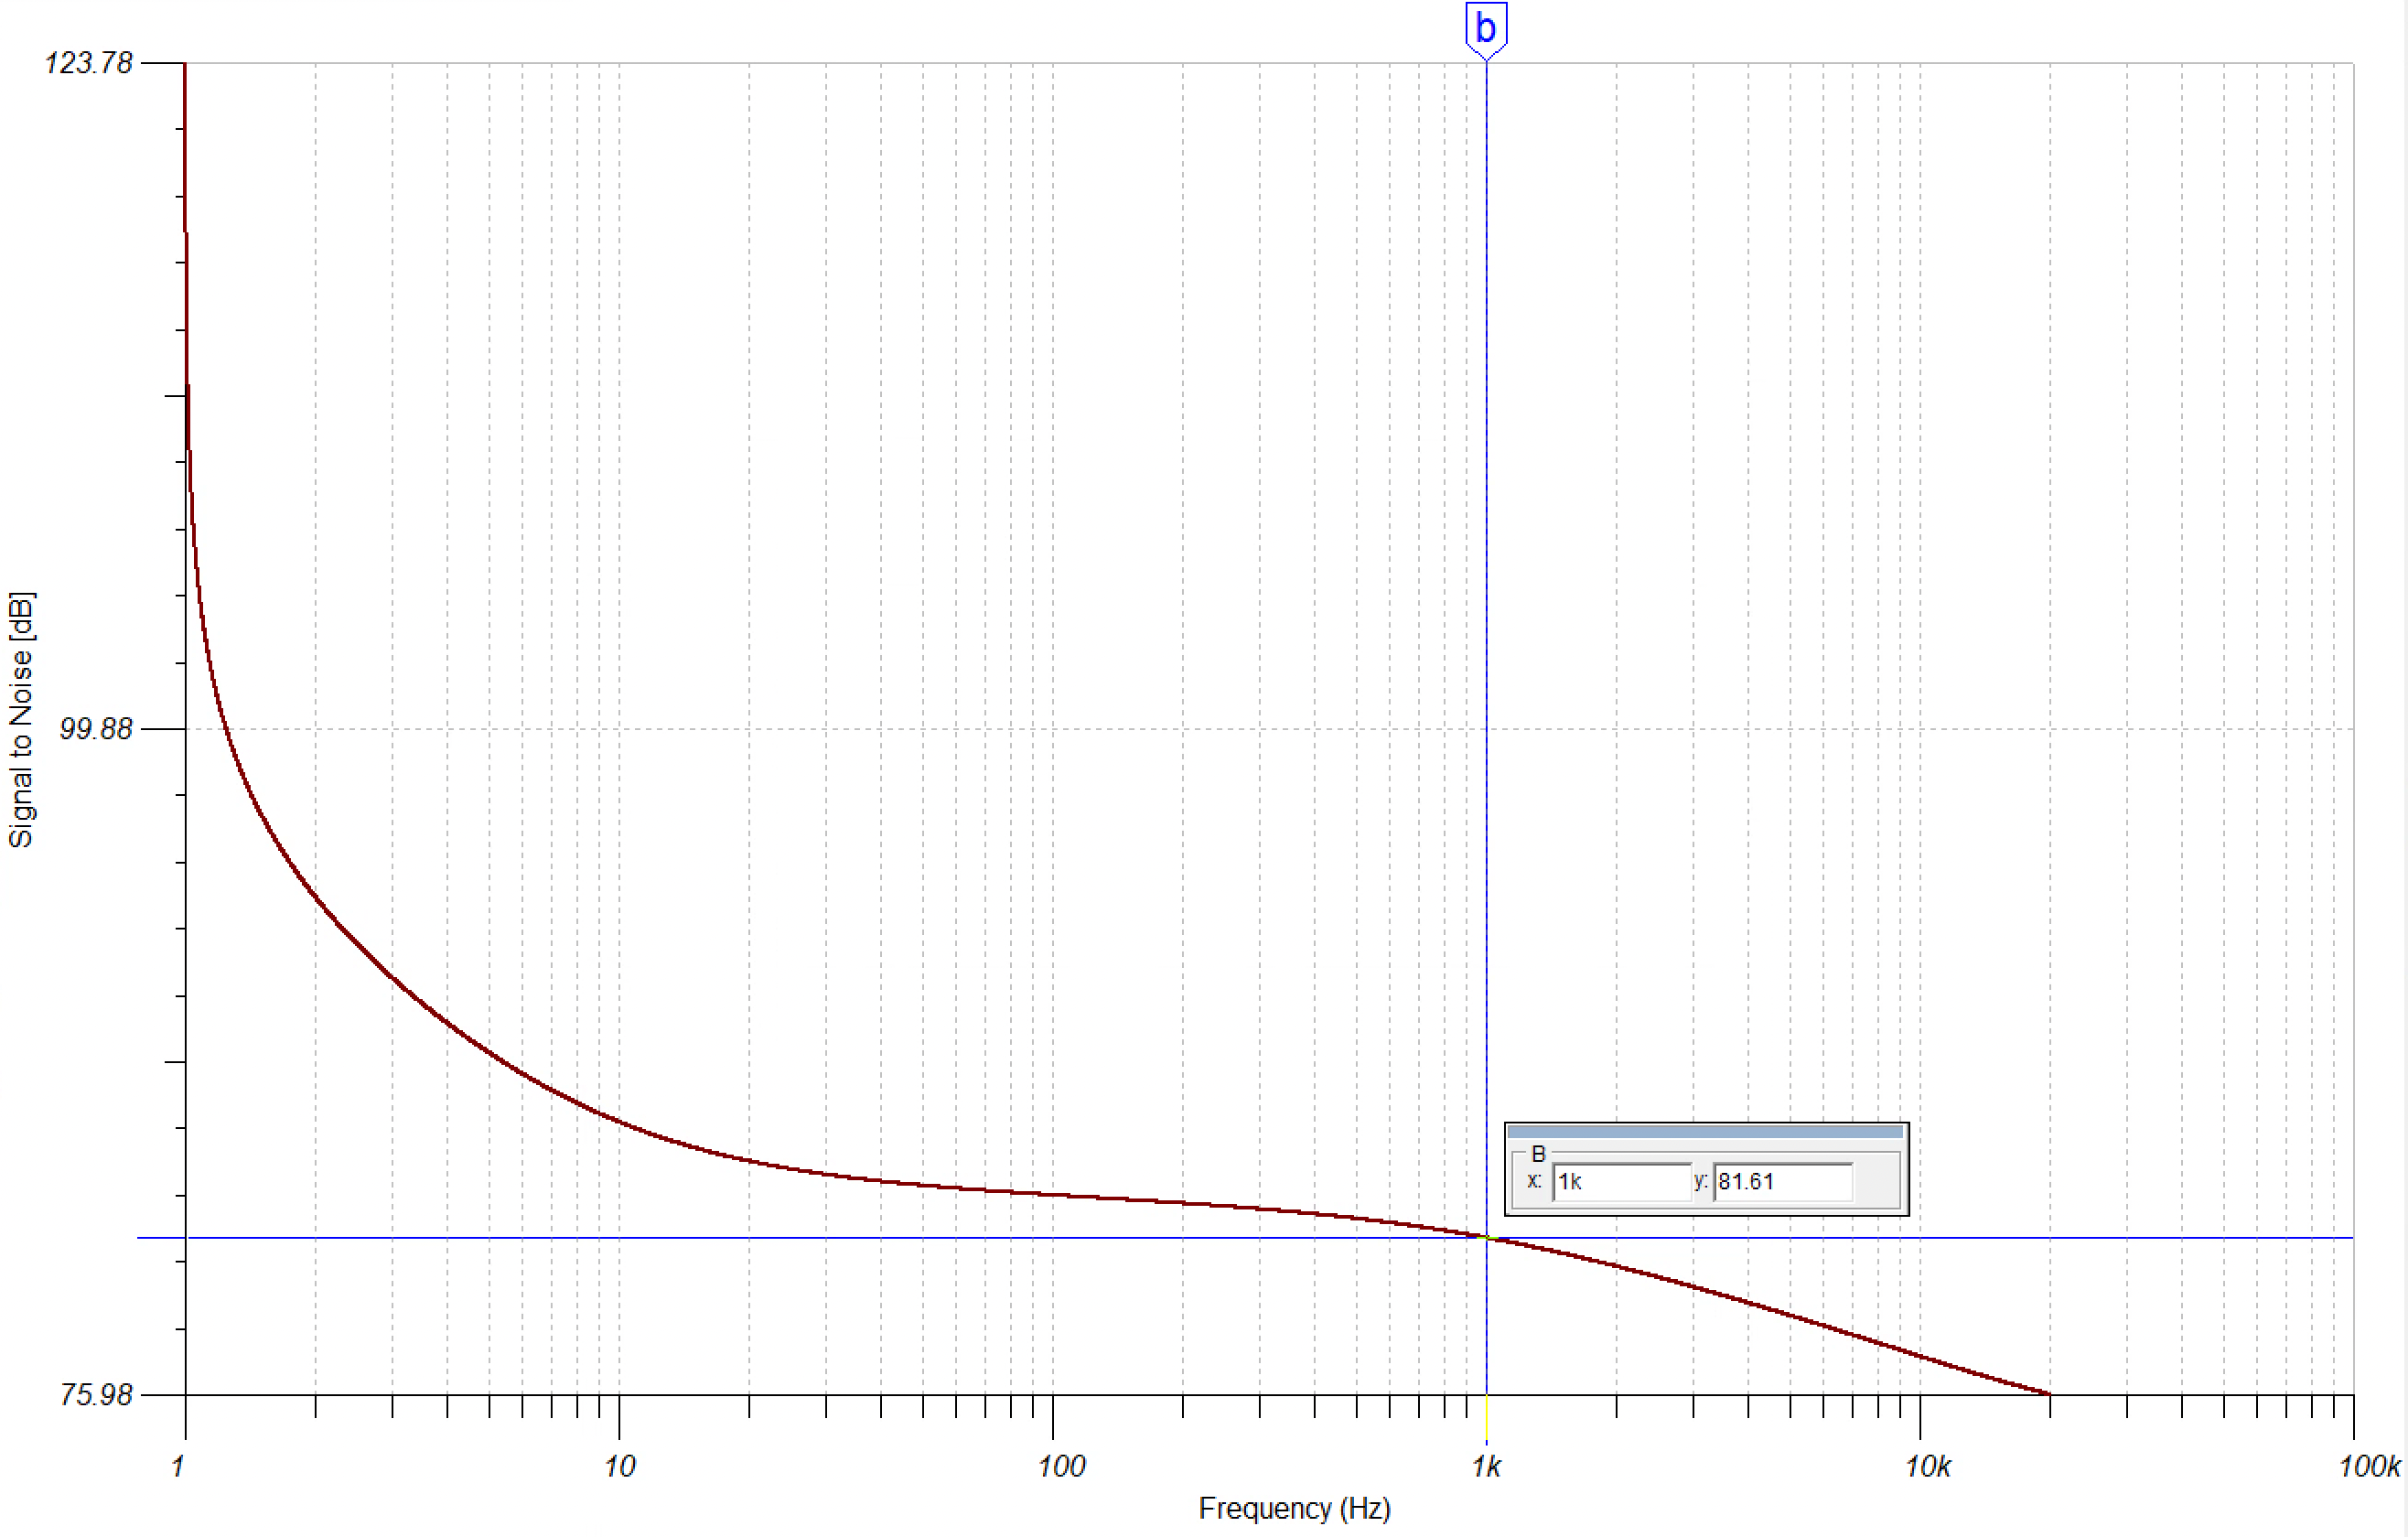
\includegraphics[width=\widthnarrow]{figures/eval/snr.png}
\caption{SNR for an output value of approximately 80~mV (corresponding to a 1~nA photocurrent at 1000~kHz).}
\label{fig:snr}
\end{figure}

\begin{figure}[t]
\centering
\includegraphics[width=\widthnarrow]{figures/eval/detectors.png}
\caption{Setup of the photodiode array used for detection.}
\label{fig:detectors}
\end{figure}

\begin{figure*}[t]
    \centering
    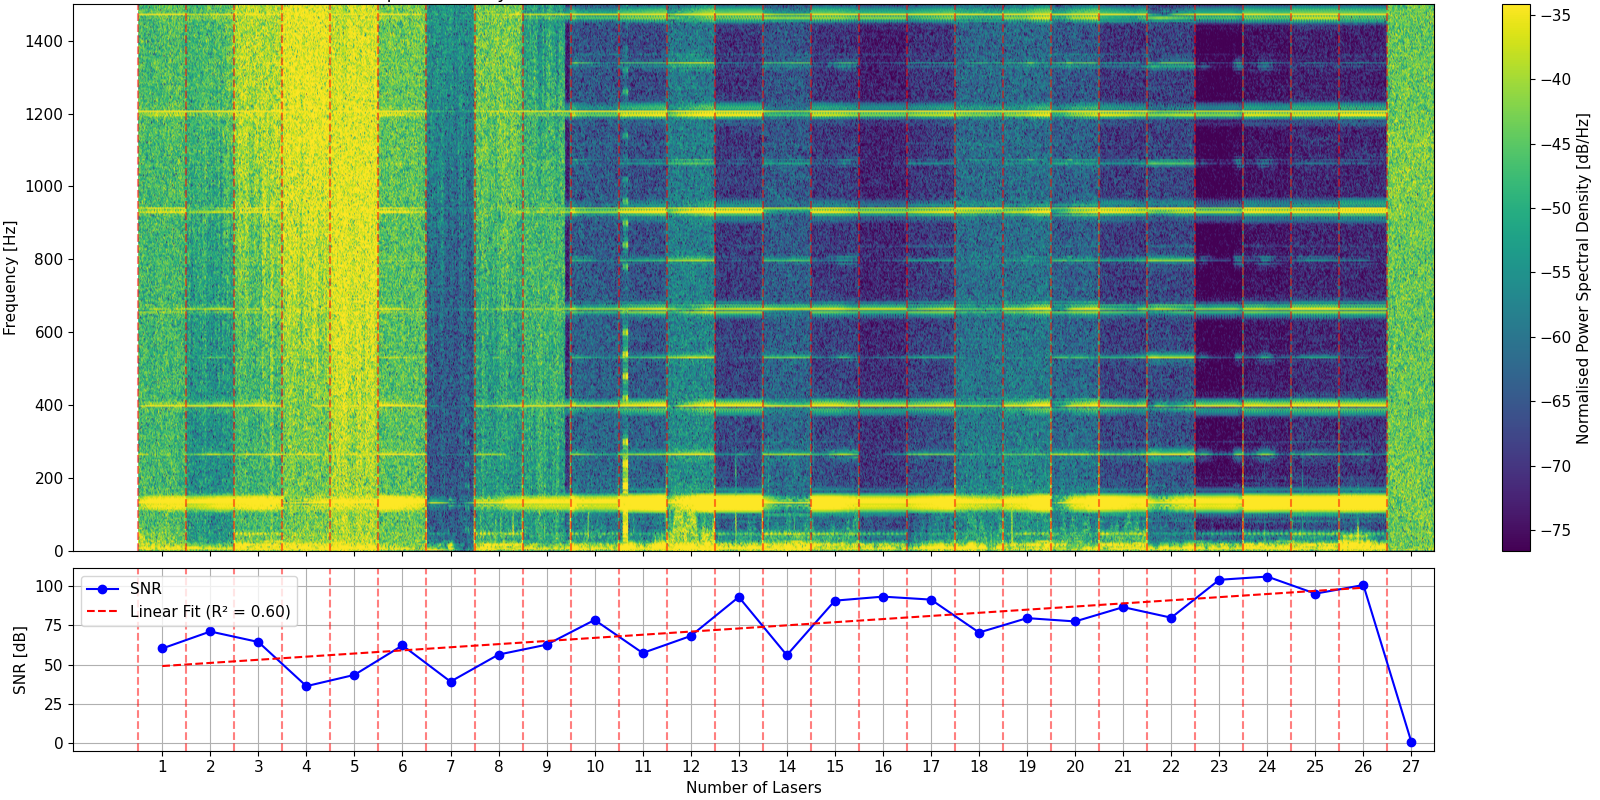
\includegraphics[width=\textwidth]{figures/results/multilaser_spectrogram}
    \caption{Spectral analysis of a 133~Hz surface vibration under different laser configurations. 
    Top: Power spectral density showing the target frequency component. Bottom: SNR improvement with increasing number of active lasers.}
    \label{fig:laser_snr}
\end{figure*}

\begin{figure*}[t]
\centering
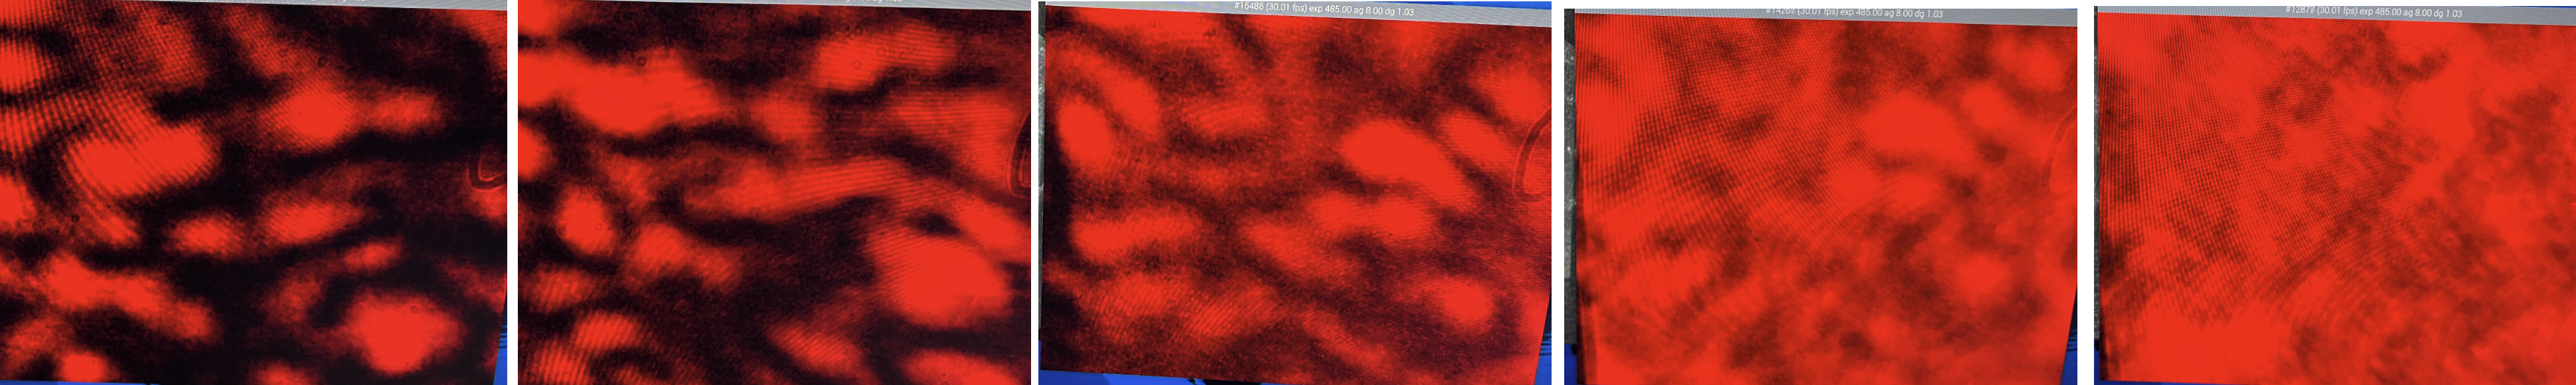
\includegraphics[width=\textwidth]{figures/eval/speckles}
\caption{Visualization of speckle patterns under different 1~mW IR laser configurations using the square laser array from Figure~\ref{fig:lasers}. Top left: 1 laser. Bottom right: 10 lasers.}
\label{fig:speckles}
\end{figure*}

\begin{figure*}[t]
\centering
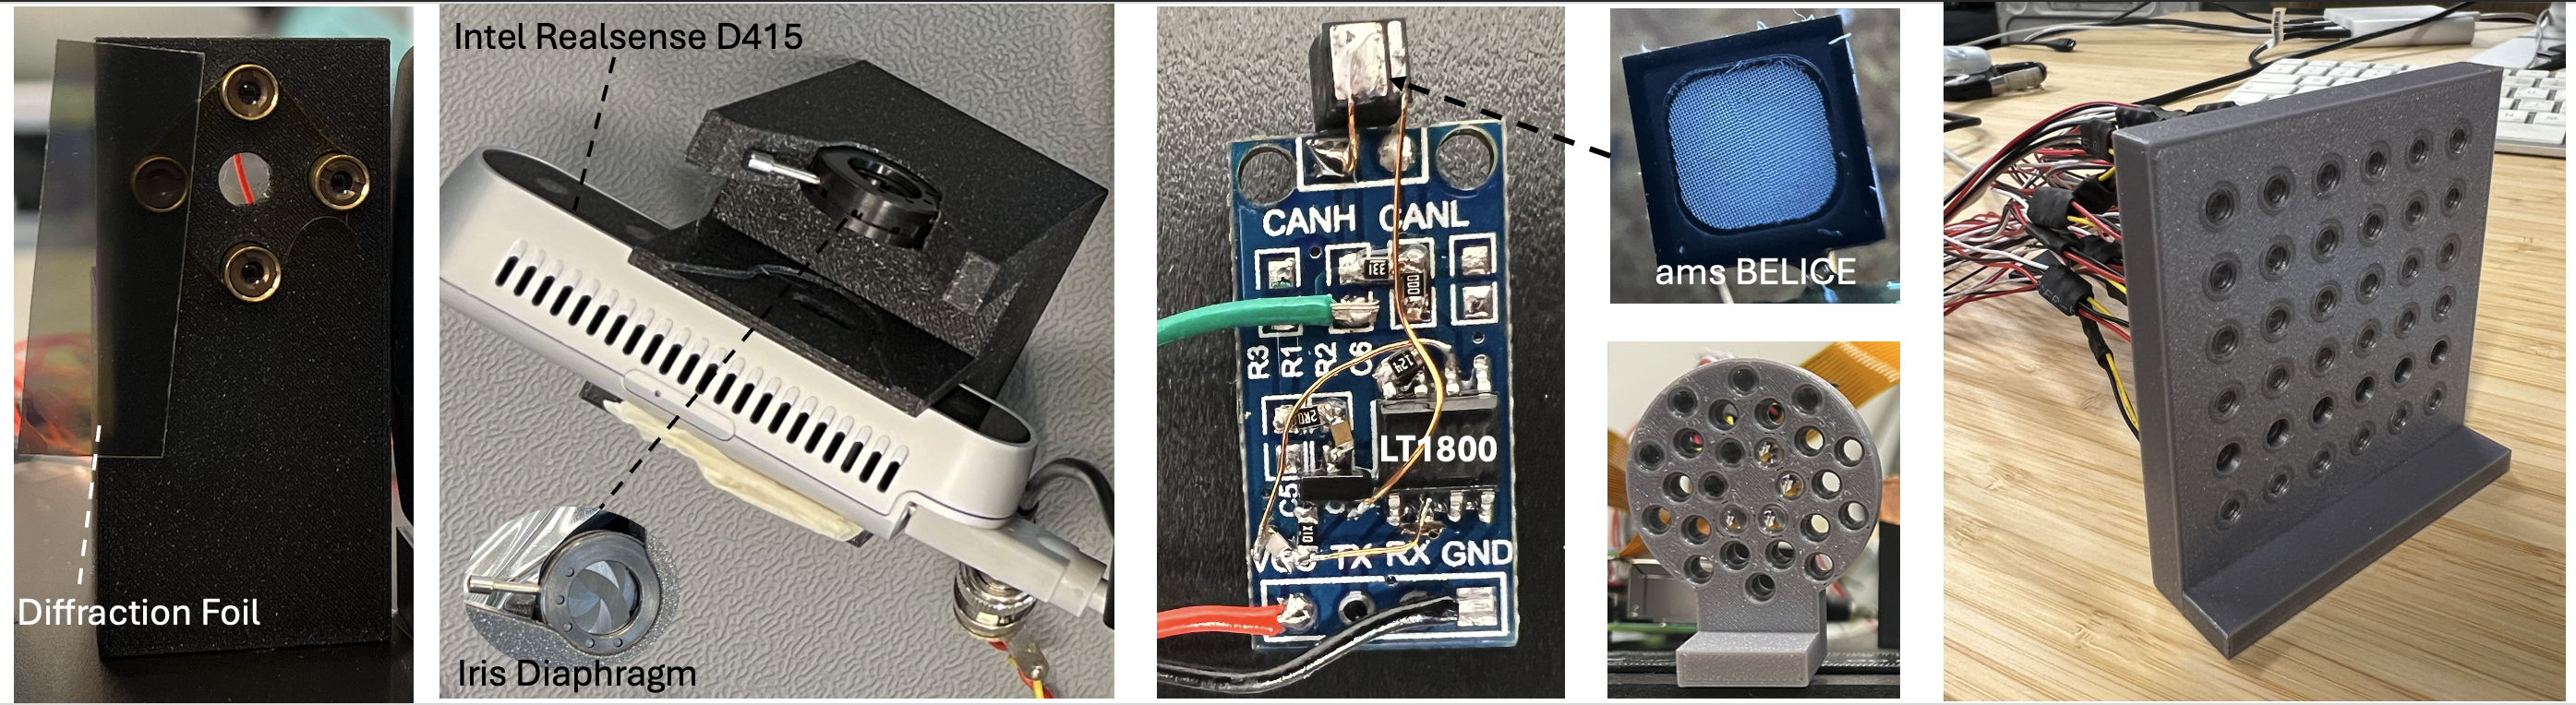
\includegraphics[width=\textwidth]{figures/eval/lasers}
\caption{The different laser setups used from left to right: Red laser for initial emulation experiments, Realsense 415 dot projector with iris, reverse engineered Realsense dot projector and driver circuit, discrete circular and square IR laser arrays.}
\label{fig:lasers}
\end{figure*}

\section{Results}
\label{sec:results}

\subsection{Speckle Motion Detection}

The results confirmed that the motion of speckle patterns was successfully detected using the discrete photodiode array. 
Phase-shifted signals were observed across multiple photodiodes, indicating the presence of a moving speckle pattern. 
This phase information confirmed that the photodiode array could effectively visualize the dynamic speckle motion. 
The use of an IR LED further validated that the detected signals originated from laser speckle patterns and not from external light interference.

\subsection{Signal-to-Noise Ratio (SNR) Analysis}

The SNR analysis demonstrated a positive correlation between the number of active lasers in the square array and the measurement quality. 
Incremental activation of the lasers resulted in an improvement in SNR, as shown in Figure~\ref{fig:laser_snr}. 
The power spectral density analysis highlighted the 133 Hz vibration component of the piezo disc, with an R² value of 0.60 indicating a moderately strong relationship between the number of lasers and SNR enhancement.

Control experiments with all lasers turned off verified that the observed signals originated from the laser speckle patterns and not from other sources. 
These results support the hypothesis that the use of multiple lasers enhances the SNR, improving the sensitivity of the system.

\subsection{Circuit Performance}

The custom-designed PCB and amplifier circuit were validated using SPICE simulations and experimental measurements. 
The Bode plot in Figure~\ref{fig:bodeplot} demonstrated a stable frequency response with high gain, while the transient response shown in Figure~\ref{fig:transient} confirmed system stability. 
Noise measurements (Figure~\ref{fig:totalnoise}) indicated a low total noise level, making the circuit suitable for laser speckle detection.

\subsection{Impact of Experimental Parameters}

The experiments revealed several critical factors impacting the measurement results. 
The PCB required thorough cleaning with IPA and compressed air to eliminate flux residue, as any remaining contaminants introduced noise. 
Additionally, conducting experiments in a light-controlled environment was essential to prevent saturation of the opamp and ensure reliable data capture. 
Dot projector alignment, facilitated by cameras, is critical for ensuring consistent speckle patterns and uniform distribution across the photodiode array.

\subsection{Limitations}
The opamp saturated in sunlight, rendering the signal irrecoverable in such conditions. Dot projectors cannot be effectively used as the reflected light is too weak.
Furthermore, the bandwidth of the system is limited to 1kHz.


\begin{figure*}[t]
    \centering
    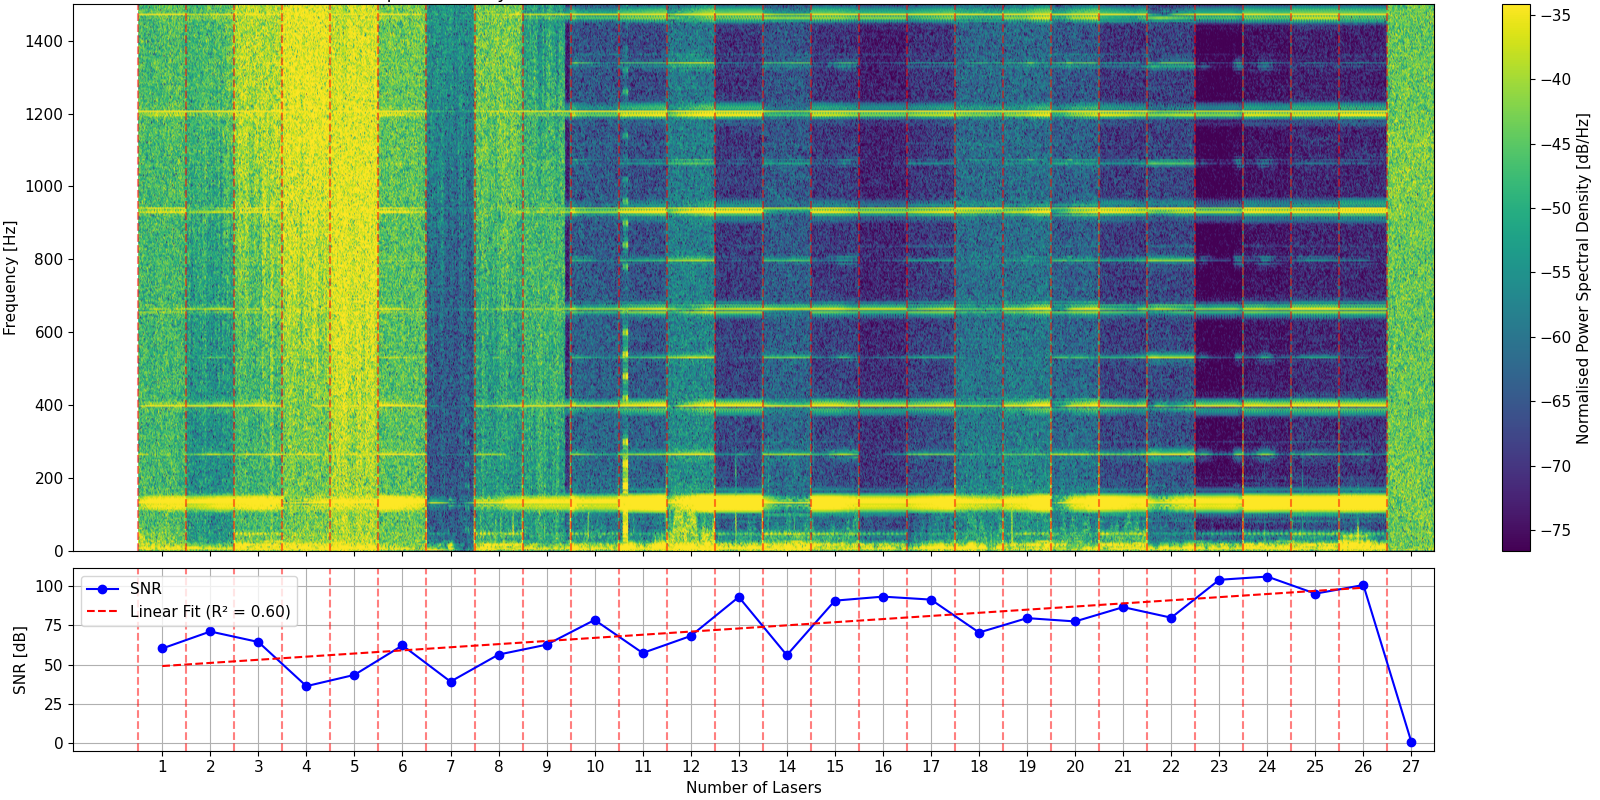
\includegraphics[width=\textwidth]{figures/results/multilaser_spectrogram}
    \caption{Spectral analysis of a 133~Hz surface vibration under different laser configurations. 
    Top: Power spectral density showing the target frequency component. Bottom: SNR improvement with increasing number of active lasers.}
    \label{fig:laser_snr}
\end{figure*}
\section{Discussion}
\label{sec:discussion}




What was surprising? unexpected? intriguing?

Were any hypotheses confirmed or rejected?

Were the predictions of any theory upheld or refuted?

What is important and worthy of again being called to the reader's attention?

What are the implications of your results?

What do they mean for this topic and your field?

Did you fulfill the promises you set out in the Introduction via the claims you made about your work?

What worked and what did not work?
\subsection{Future Work}
\label{sub:future_work}

To address the identified limitations and improve the system, several avenues for future work are proposed:

\begin{itemize}
    \item \textbf{Higher Bandwidth}: Replace the current opamp with one that has a higher gain-bandwidth product (GBW) to increase the system bandwidth and enable detection of faster speckle movements.
    \item \textbf{Current to Digital Amp}: Integrate a current-to-digital amplifier chip, such as the DDC118, to enhance system integration and make the PCB smaller.
    \item \textbf{Sensor Vibration Compensation}: Mitigate the influence of vibrations from the sensor itself by incorporating an accelerometer to subtract self-induced motion artifacts from the measurements.
    \item \textbf{Synchrous Detection}: Modulate the laser light with a known reference signal to perform synchronous detection (aka lock-in amplifier) for more robustness against daylight.
\end{itemize}
\section{Acknowledgments}
\label{sec:acknowledgments}

I would like to thank Professor Christian Holz and Paul Streli for the opportunity to work on this project in the Sensing, Interaction \& Perception Lab, and for their valuable feedback throughout its development. 
Their guidance and insights helped shape this work.
Special thanks to Dr. Johannes Wüthrich and Raffael Tschui for many helpful discussions and brainstorming sessions that helped chew through ideas.
I am also grateful to Jan Hug for his thorough proofreading and suggestions that improved this thesis.

% balance columns on last page
\balance{}

\bibliography{references}

\clearpage 
\onecolumn
\appendix

\section{Experimental Setups}
\label{sec:experimental-setups}

This appendix documents the experimental setups used throughout this work. The figures are organized as follows:

\begin{itemize}
  \item Figures \ref{fig:cam1} and \ref{fig:cam2} show the initial camera setup used to visualize and validate speckle patterns.
  \item Figure \ref{fig:detectors} presents the different detectors used for alignment and baseline measurements.
  \item Figure \ref{fig:speckles} demonstrates how speckle patterns vary with different laser configurations.
  \item Figure \ref{fig:setup} shows the final experimental setup with the piezo disc.
  \item Figure \ref{fig:lasers} documents the various laser configurations developed during this work.
  \item Figure \ref{fig:config} visualises the speckle pattern for each laser configuration used.
\end{itemize}

\begin{figure}[t]
\centering
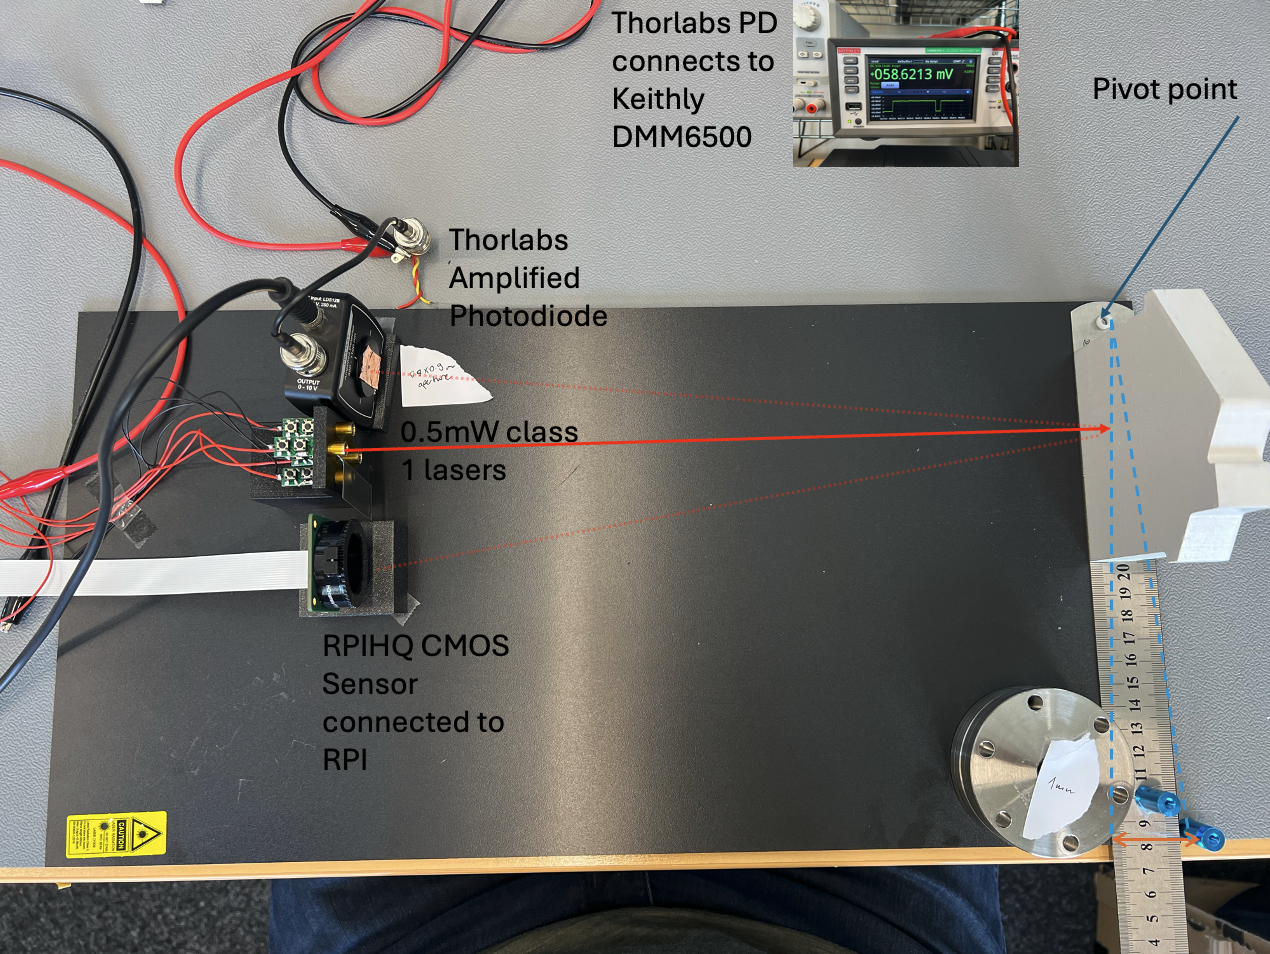
\includegraphics[width=\textwidth]{figures/impl/camera_setup.png}
\caption{A laser is pointed at a painted wooden surface. A multimeter measured the current from a masked photodiode. 
A RPI HQ camera is used as a reference to visualise the speckle pattern.}
\label{fig:cam1}
\end{figure}

\begin{figure}[t]
\centering
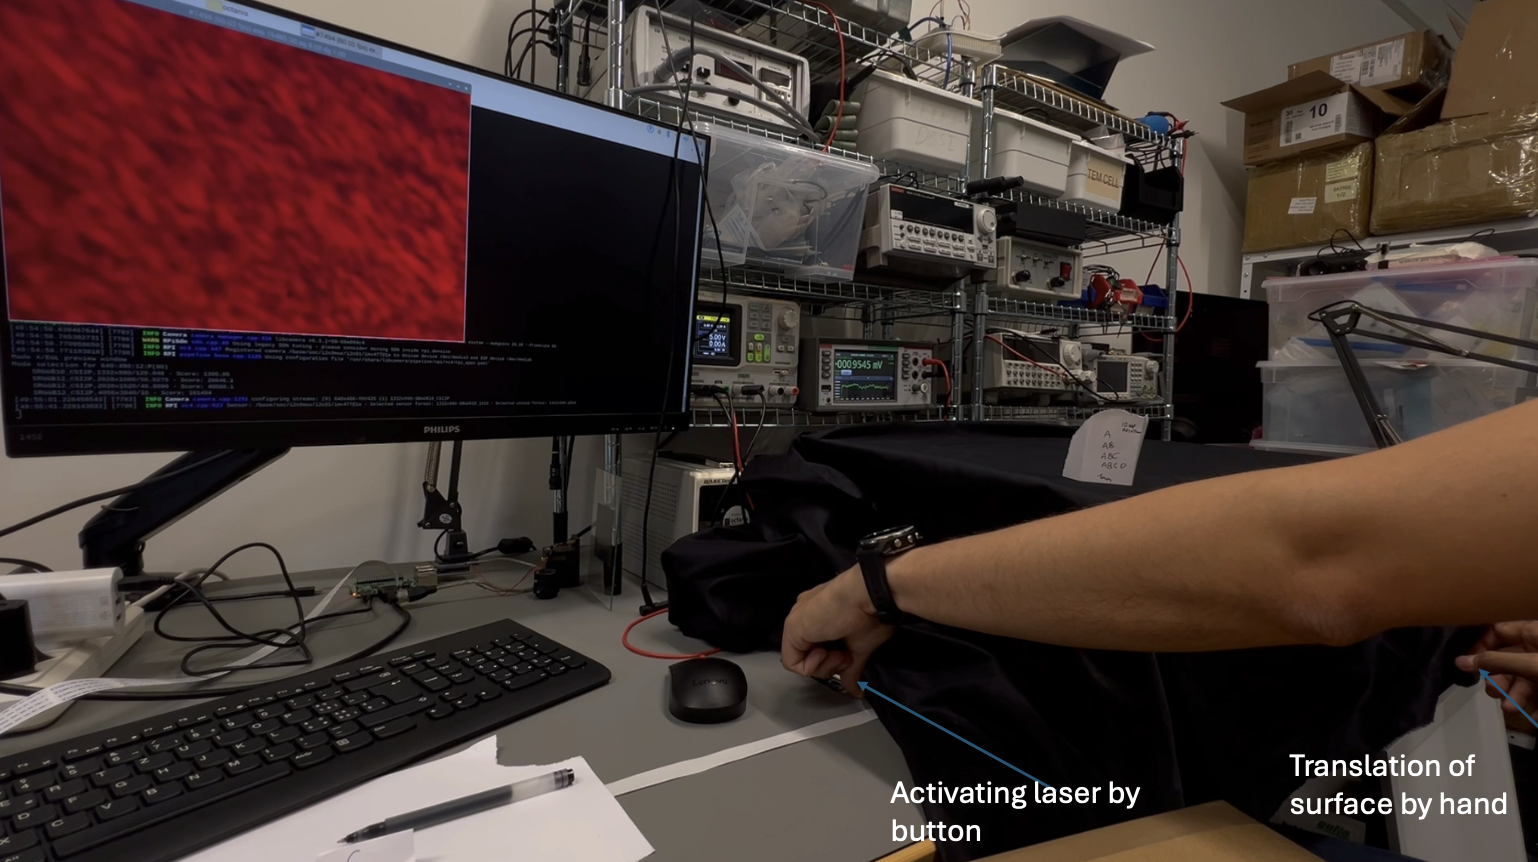
\includegraphics[width=\textwidth]{figures/impl/camera_setup2.png}
\caption{Speckle pattern visualised by RPI Cam HQ (from Setup in Figure \ref{fig:cam1})}
\label{fig:cam2}
\end{figure}

\begin{figure}[t]
\centering
\includegraphics[width=\widthnarrow]{figures/eval/detectors.png}
\caption{The Raspberry Pi No-IR (top left) was used to align invisible IR lasers, the Raspberry Pi HQ camera for 
showing speckle patterns and the (masked) Thorlabs detector for establishing a photocurrent baseline for our amplifier.}
\label{fig:detectors}
\end{figure}

\begin{figure*}[t]
\centering
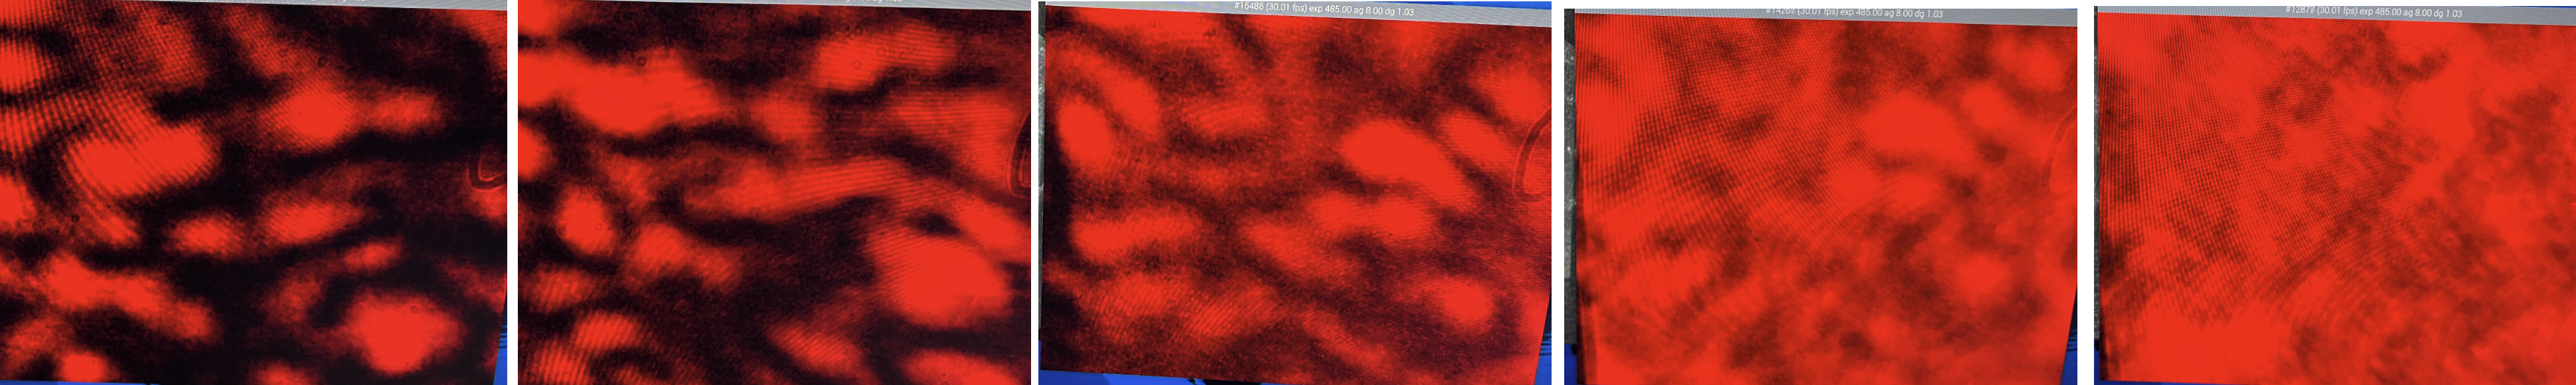
\includegraphics[width=\textwidth]{figures/eval/speckles}
\caption{Visualization of speckle patterns under different 1~mW IR laser configurations using the square 
laser array from Figure~\ref{fig:lasers}. Top left: 1 laser. Bottom right: 10 lasers.}
\label{fig:speckles}
\end{figure*}

\begin{figure*}[t]
\centering
\includegraphics[width=\textwidth]{figures/eval/typical_setup.png}
\caption{Photo of the experimental configuration with the piezo disc.}
\label{fig:setup}
\end{figure*}

\begin{figure*}[t]
\centering
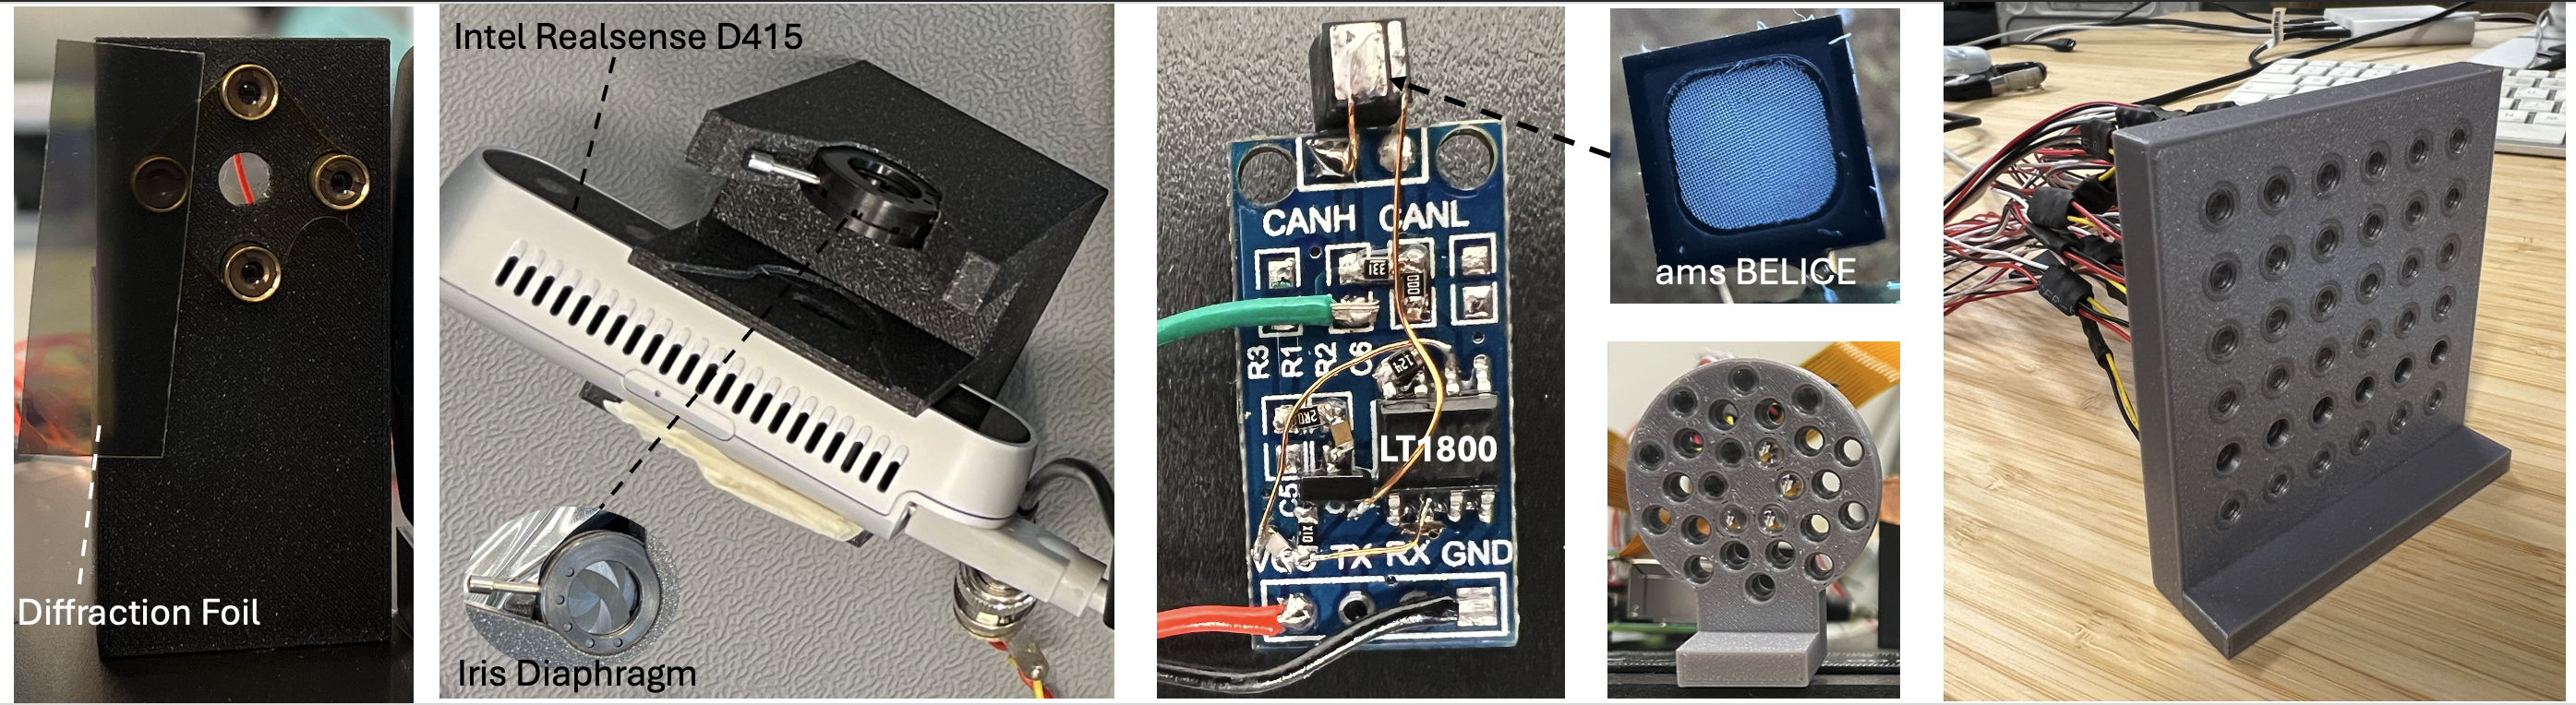
\includegraphics[width=\textwidth]{figures/eval/lasers}
\caption{The different laser setups used from left to right: Red laser for initial emulation experiments, 
Realsense 415 dot projector with iris, reverse engineered Realsense dot projector and driver circuit, 
discrete circular and square IR laser arrays.}
\label{fig:lasers}
\end{figure*}

    

\begin{figure*}[t]
\centering
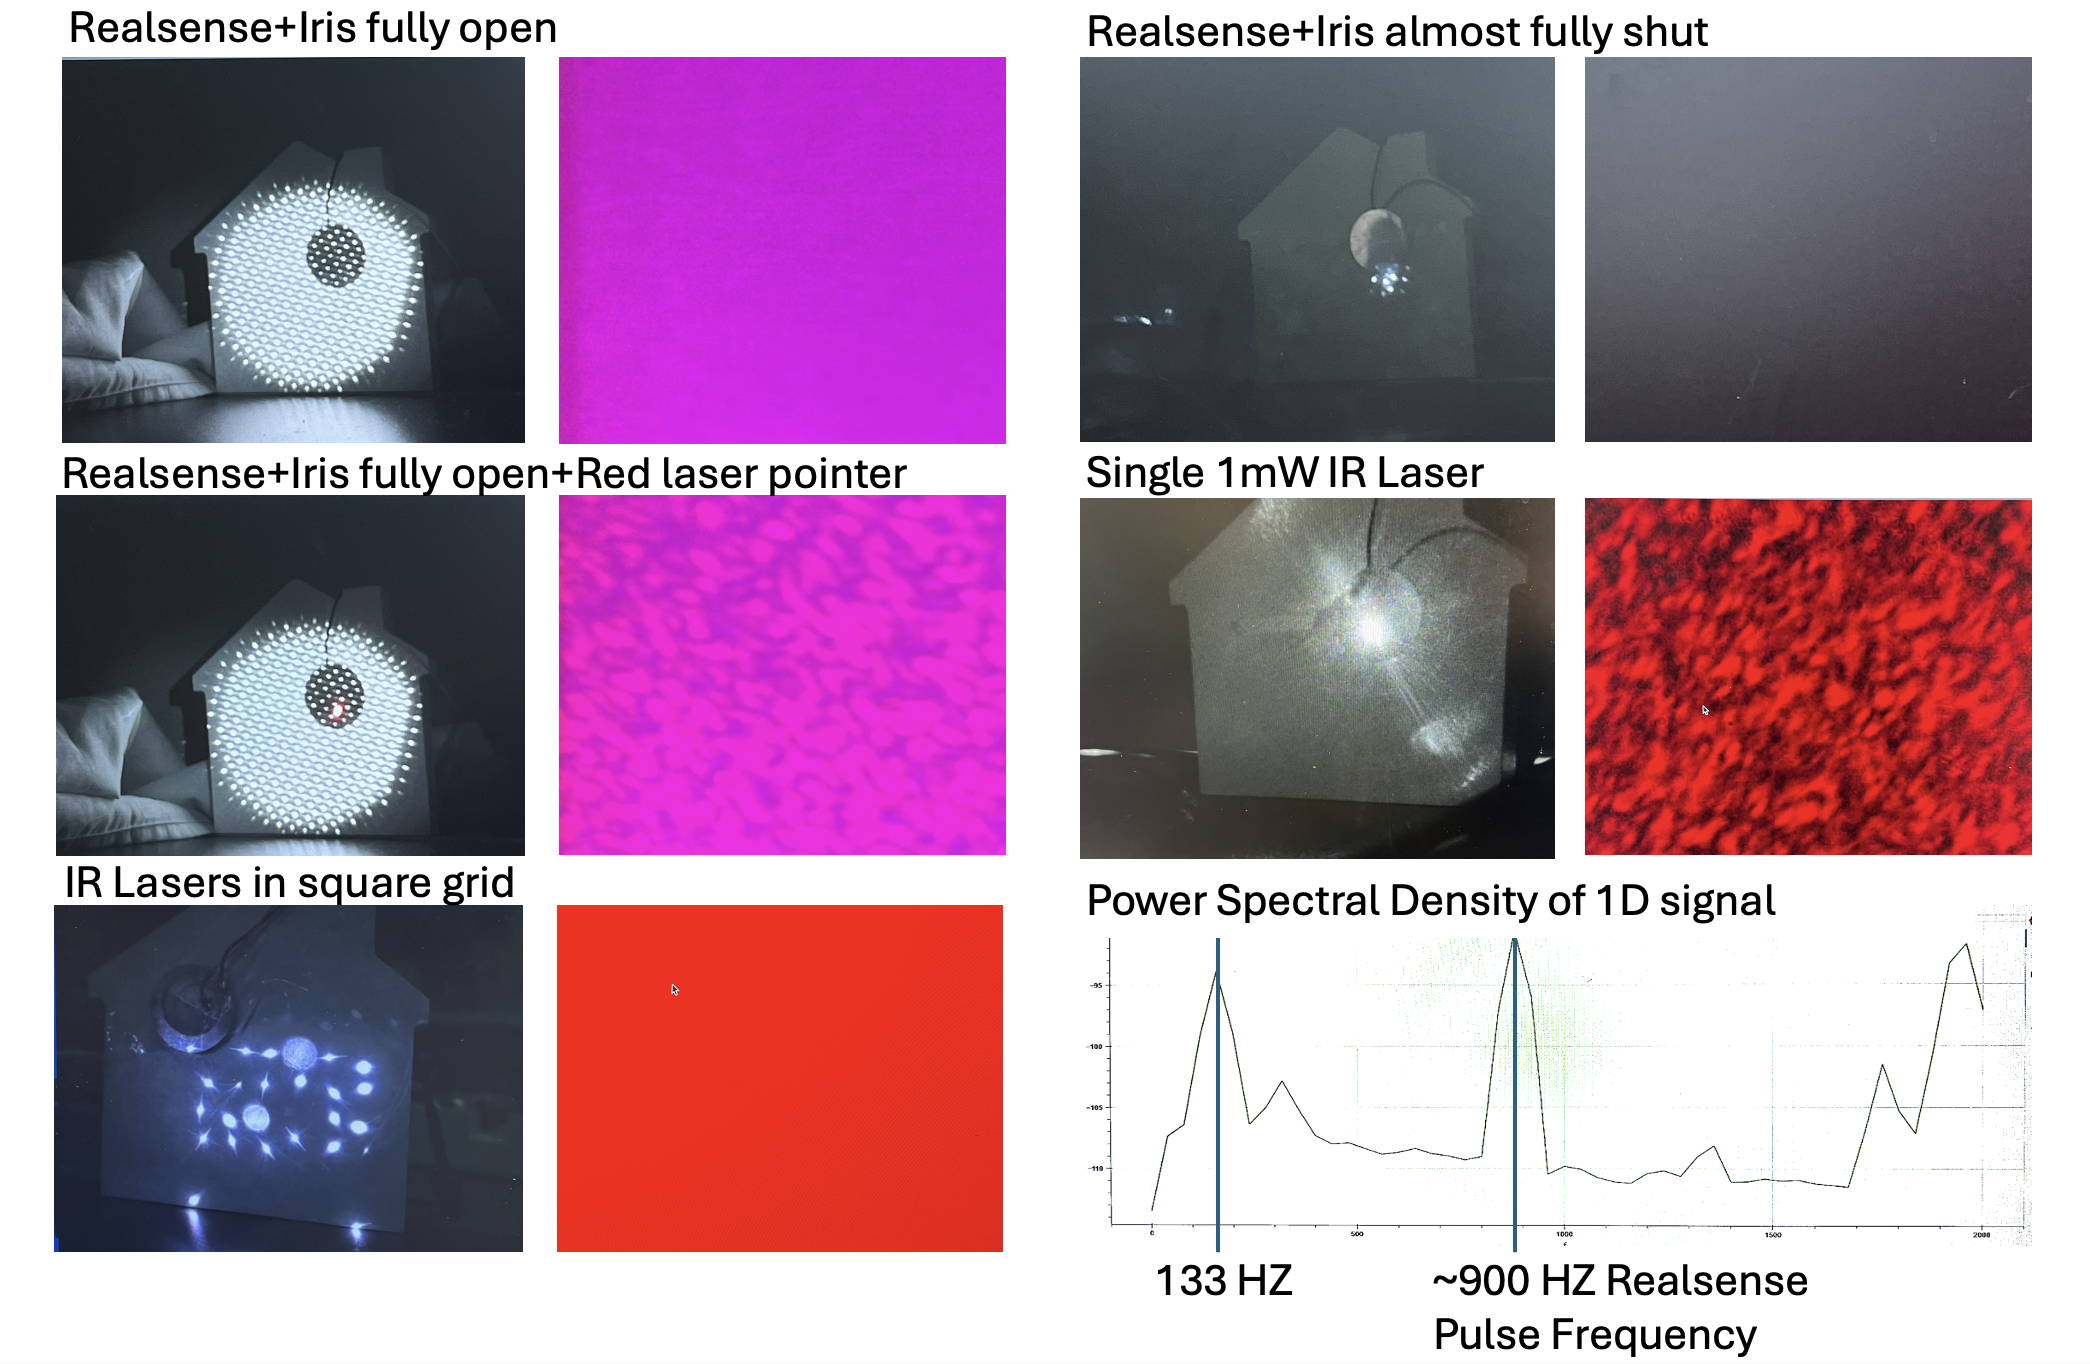
\includegraphics[width=\textwidth]{figures/results/configs}
\caption{Laser configuration and resulting speckle patterns on the camera sensor. Bottom right shows the PSD of the 1d signal. When the Realsense is used, we see a peak at 900 Hz due to the pulsing nature of the dot projector. Note that our detector can only pick up the Realsense speckle pattern if and only if the surface has high reflectivity and is aligned perfectly. The square grid lasers are somewhat distorted, due to mechanical stress on the low grade plastic collimating lenses used.}
\label{fig:config}
\end{figure*}

\begin{figure*}[t]
\centering
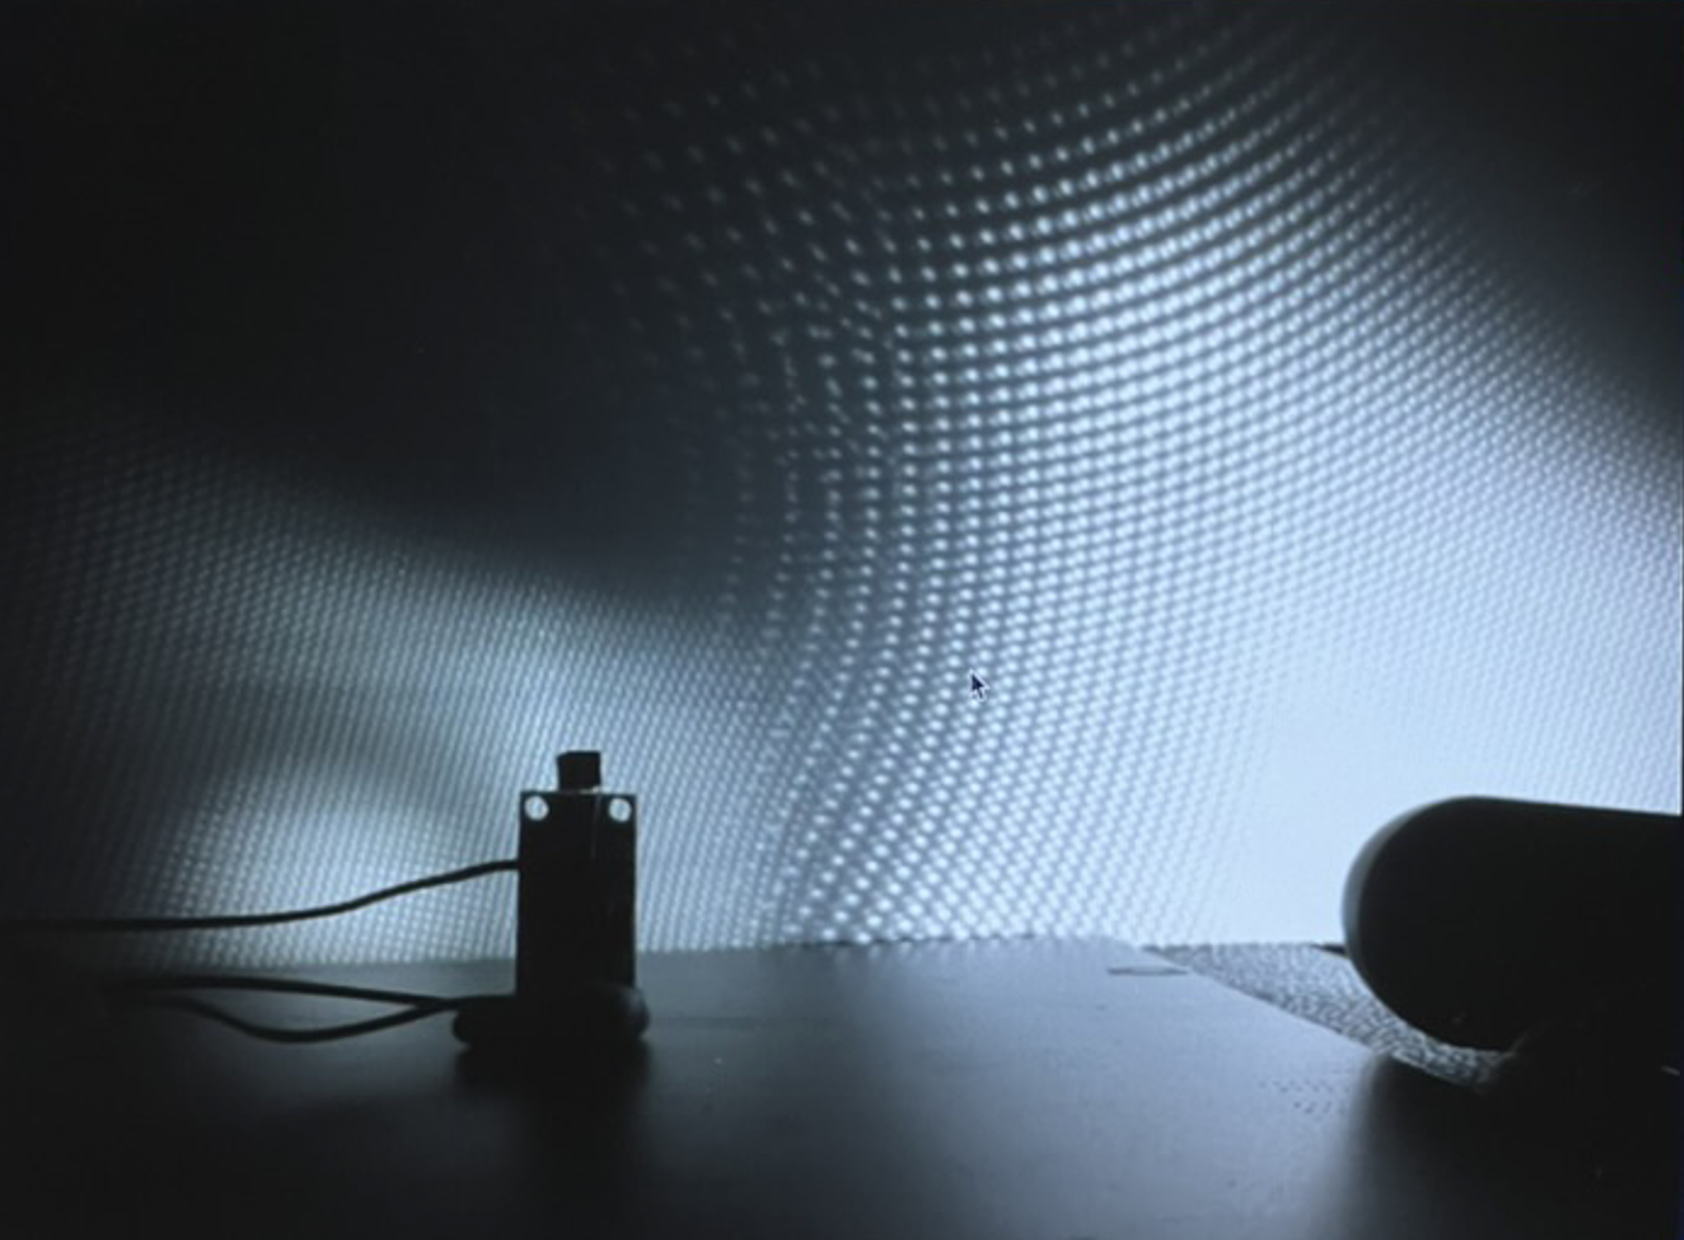
\includegraphics[width=\textwidth]{figures/results/rsvsdiy}
\caption{Our dot  project vs the Realsense camera. The pattern seams different, but this is due to the Realsense using 2 side by side dot projectors. If we cover up one, we get an identical pattern.}
\label{fig:rsvsdiy}
\end{figure*}
    
\onecolumn 

\end{document}
